%%% File encoding: UTF-8
%% äöüÄÖÜß  <-- no German Umlauts here? Use an UTF-8 compatible editor!

%%% Magic comments for setting the correct parameters in compatible IDEs
% !TeX encoding = utf8
% !TeX program = pdflatex 
% !TeX spellcheck = en_US
% !BIB program = biber

\documentclass[master,english]{hgbthesis}
% Permissible options in [..]: 
%   Type of work: diploma, master (default), bachelor, internship 
%   Main language: german, english (default)
%%%----------------------------------------------------------

\RequirePackage[utf8]{inputenc}		% Remove when using lualatex or xelatex entfernen!

\graphicspath{{images/}}    % location of images and graphics
\logofile{logo}				% logo file = images/logo.pdf (use \logofile{} for no logo)
\bibliography{references}  	% name of bibliography file (references.bib)

%%%----------------------------------------------------------
% Title page entries
%%%----------------------------------------------------------

%%% Entries for ALL types of work: --------------------------
\author{Anna M.\ Maureder}
\title{IM690 Thesis Project 1\\ % the name of the course or project
	Unsupervised Identification of the rigid parts of an unknown articulated object}	% or "Term Report"
\programname{Interactive Media}
\placeofstudy{Hagenberg}
\dateofsubmission{2017}{02}{28}	% {YYYY}{MM}{DD}

%%% Entries for Bachelor theses only: -----------------------
\thesisnumber{XXXXXXXXXX-A}   %e.g. 1310238045-A  
% (Stud-ID, A = 1st Bachelor thesis)
\semester{Fall Semester 2017} 	% Fall/Spring Semester YYYY
\coursetitle{Introduction to Trivial Problems 1} 
\advisor{Roger K.~Putnik, M.Sc.}

%%% Restricted publication license instead of CC (master only):
%\strictlicense

%%%----------------------------------------------------------
\begin{document}
%%%----------------------------------------------------------

%%%----------------------------------------------------------
\frontmatter							% title part (roman page numbers)
%%%----------------------------------------------------------

\maketitle
\tableofcontents

\chapter{Preface}






 	% preface is optional
\chapter{Abstract}


The proposed work describes a method for pose estimation of articulated objects without any prior knowledge of their body parts. Most existing pose estimation methods take advantage of trackers, and user inputs to estimate the joint positions. However, a completely unsupervised method constitutes an enormous potential but also a great challenge. A main solution to that is proposed by template matching associated with the non-rigid registration of meshes, which requires two poses of the same object and applies the Expectation-Maximization algorithm to segment the object into its rigid parts. This is done iteratively by assigning mesh points on body parts and finding transformations that perfectly match those body parts on both meshes. Based on this approach, a segmentation method is developed to obtain the rigid parts of an object and consequently estimate its joints.


\chapter{Kurzfassung}

\begin{german}
An dieser Stelle steht eine Zusammenfassung der Arbeit in Deutsch.
\end{german}

%%%----------------------------------------------------------
\mainmatter          			% main part (arabic page numbers)
%%%----------------------------------------------------------

\chapter{Introduction}
\label{cha:Introduction}
Pose and motion estimation of articulated objects is a fundamental task in computer vision due to the progressive digitalization of day-to-day processes. A variety of practical applications exist, such as activity recognition, video surveillance and human-computer interfaces. A case of application the thesis emerged from is the pose capture of a real world articulated object used as input for a digital animation process. Thereby, the principal goal is to detect associated rigid parts and joints in two consecutive poses, in order to interpolate the animation between transformed rigid parts.

\section{Problem statement}
Generally, pose estimation of an articulated object can be described as a segmentation problem as the individual rigid parts and joints linking them are desired. A vast majority of existing pose estimation approaches take advantage of assumed object models in 3D and manually labeled joints and rigid parts to determine basic information about an object's pose. Often combined with a machine learning approach the results are promising after a completed training phase. However, unsupervised methods that detect the pose of an unknown object, constitute a great potential as the pose estimation operates completely independent from user input. Among those methods, the non-rigid registration (see section \ref{registration}) is a well-known approach. The input of this algorithm are two or more poses of one articulated object. By merging one \textit{template} pose onto another \textit{query} pose, part correspondences can be determined and the articulated object is segmented into its rigid parts. 
By applying this approach to an unknown input object in two poses, five core questions are formulated to be considered:
%%
\\\begin{itemize}
	\item How and in which form is the input data for pose estimation received?
	\item Which data points correspond to each other in two different poses?
	\item To which rigid part can a data point be assigned to?
	\item How to estimate the joints linking detected rigid parts?
	\item Which joints/rigid parts correspond to each other in two different poses?
\end{itemize}
%%
Many challenges have to be overcome emerging from different stages of the pose estimation procedure (see section \ref{poseEstimation}). To name the most crucial ones, digital input data of an articulated object in the real world has to be captured. Thereby, input noise emerging from low resolution scanning technologies is an essential factor which has to be considered for pose estimation. Furthermore, the ambiguity of body parts poses a significant difficulty especially if the articulated object is composed of symmetric body parts. One of the main drawbacks of current methods is the computational expensive procedure to detect rigid parts. The root of this problem originates from the detection of correct point correspondences between two input meshes. As this directly influences the run time there is a great demand for improvements, especially if real-time applications are required.

\section{Goal}
By means of current approaches in this particular field (see chapter \ref{cha:StateOfTheArt}), my thesis addresses the issue to detect the initial pose of an unknown articulated object given in two poses. The focus lies thereby on reducing the computation steps of the segmentation procedure. Assuming, a digitalized model in form of the object's hull is available, the thesis fully focuses on the segmentation of an articulated object into its rigid parts. The digitalization of the real world object is therefore passed over. The main goal can be formulated as segmenting an articulated object $M$ into its unknown number $n$ of rigid parts $\mathcal{P} =  \{P_1,\ldots,P_n\}$ and extract all joints $m$ $\mathcal{J} =  \{J_1,\ldots,J_m\}$ linking those parts. The input poses are represented by two 2D point clouds $C_1$ and $C_2$ of $M$ in two different poses. $C_1$ is thereby used as a \textit{template} to be registered with $C_2$. The main task is to determine a part assignment $P_i$ and the corresponding transformation $T_i$ for all points of the \textit{template} that aligns them with all points of $C_2$. The main difficulty is that only the unsorted points of $C_1$ and $C_2$ are present. No further information, like manual labeling by the user or an object model as indicator for the number of rigid parts, are available. The only assumption that can be made is that $M$ only consists of rigid parts that can not be deformed or stretched. Comparing two poses being adopted by the articulated object, the geodesic distance $g(\boldsymbol{p}_i,\boldsymbol{p}_j)$ between two mesh points $\boldsymbol{p}_i(x,y)$ and $\boldsymbol{p}_j(x,y)$ remains constant. It is also taken advantage of the knowledge that points located on a rigid part $P_i$ undergo the same transformation $T_i$.

%TODO: method
\section{Methodology}
To accomplish the proposed goal, an analysis of different pose estimation approaches is conducted in chapter \ref{cha:StateOfTheArt}. Additionally, the concept of surface registration is presented (see section \ref{registration}) to provide necessary background knowledge on segmentation. Consequently, two segmentation approaches are implemented taking unsupervised methods (see subsection \ref{unsupervised}) into consideration. Although the referred pose estimation approaches are perform on 3D data sets, it was a conscious decision to conduct the implementation on 2D point clouds. The main advantages include less degrees of freedom of the data points and a possible pose estimation in the absence of 3D reconstructed data. Furthermore, the attention can be brought to an implementation of potential improvements.

The first approach is a straightforward and linear method (see chapter \ref{cha:LinearApproach}) which aims to reduce the computation steps of previous approaches. This is achieved by iteratively subdividing $C_1$ and $C_2$ with a ``divide and conquer'' approach. Corresponding sub clusters are verified to match and in a negative case further subdivided. This attempt does only depend on all point coordinates of $C_1$ and $C_2$ and the orientation of clusters. In case of many linked parts or too dissimilar transformations between $C_1$ and $C_2$ this approach is not reliable as clusters being compared are actually not corresponding to each other. To address the segmentation with focus on articulated objects with a typical skeleton structure (e.g. a human), a feature-based approach (see chapter \ref{cha:FeatureApproach}) is implemented. In this case additional descriptors are extracted for all points of $C_1$ and $C_2$. Those assist on the initial alignment of the input clusters to detect a reliable corresponding rigid part. Proceeding from there, joints can be estimated and all linked rigid parts are detected iteratively. The main reference paper for this approach is from Guo et al \cite{guo2016correspondence}. By demonstrating the outcomes from the proposed approaches (see section \ref{ResultsLRP}) emerged drawbacks, main difficulties and possible potentials are outlined. Furthermore, planned future work is proposed to compensate originated difficulties (see chapter \ref{cha:Conclusion}). All those offer a solid base for further improvements in this area. 





\chapter{Related work}
\label{cha:RelatedWork}

By focusing on approaches computing the segmentation of articulated objects from 3D data, many different ones could be detected. They face similar challenges (see subsection \ref{Challenges}) but solve them in different ways
%%
\section{Correlated Correspondence}

A main approach for non-rigid registration is proposed by Anguelov \cite{Anguelov04} applying the correlated correspondence algorithm \cite{CorrelatedCorrespondance}. The algorithm takes a \textit{template} Mesh $D_0$ and other Meshes $D_1,\ldots,D_n$ in different configurations as input. The algorithm then performs a probabilistic framework and Expectation-Maximization (EM) to iterate between finding a decomposition of the \textit{template} into rigid parts and detecting them in the other meshes. Furthermore, a random clustering is applied to facilitate the detection of associated rigid parts.
%%
\begin{figure}
	\centering
	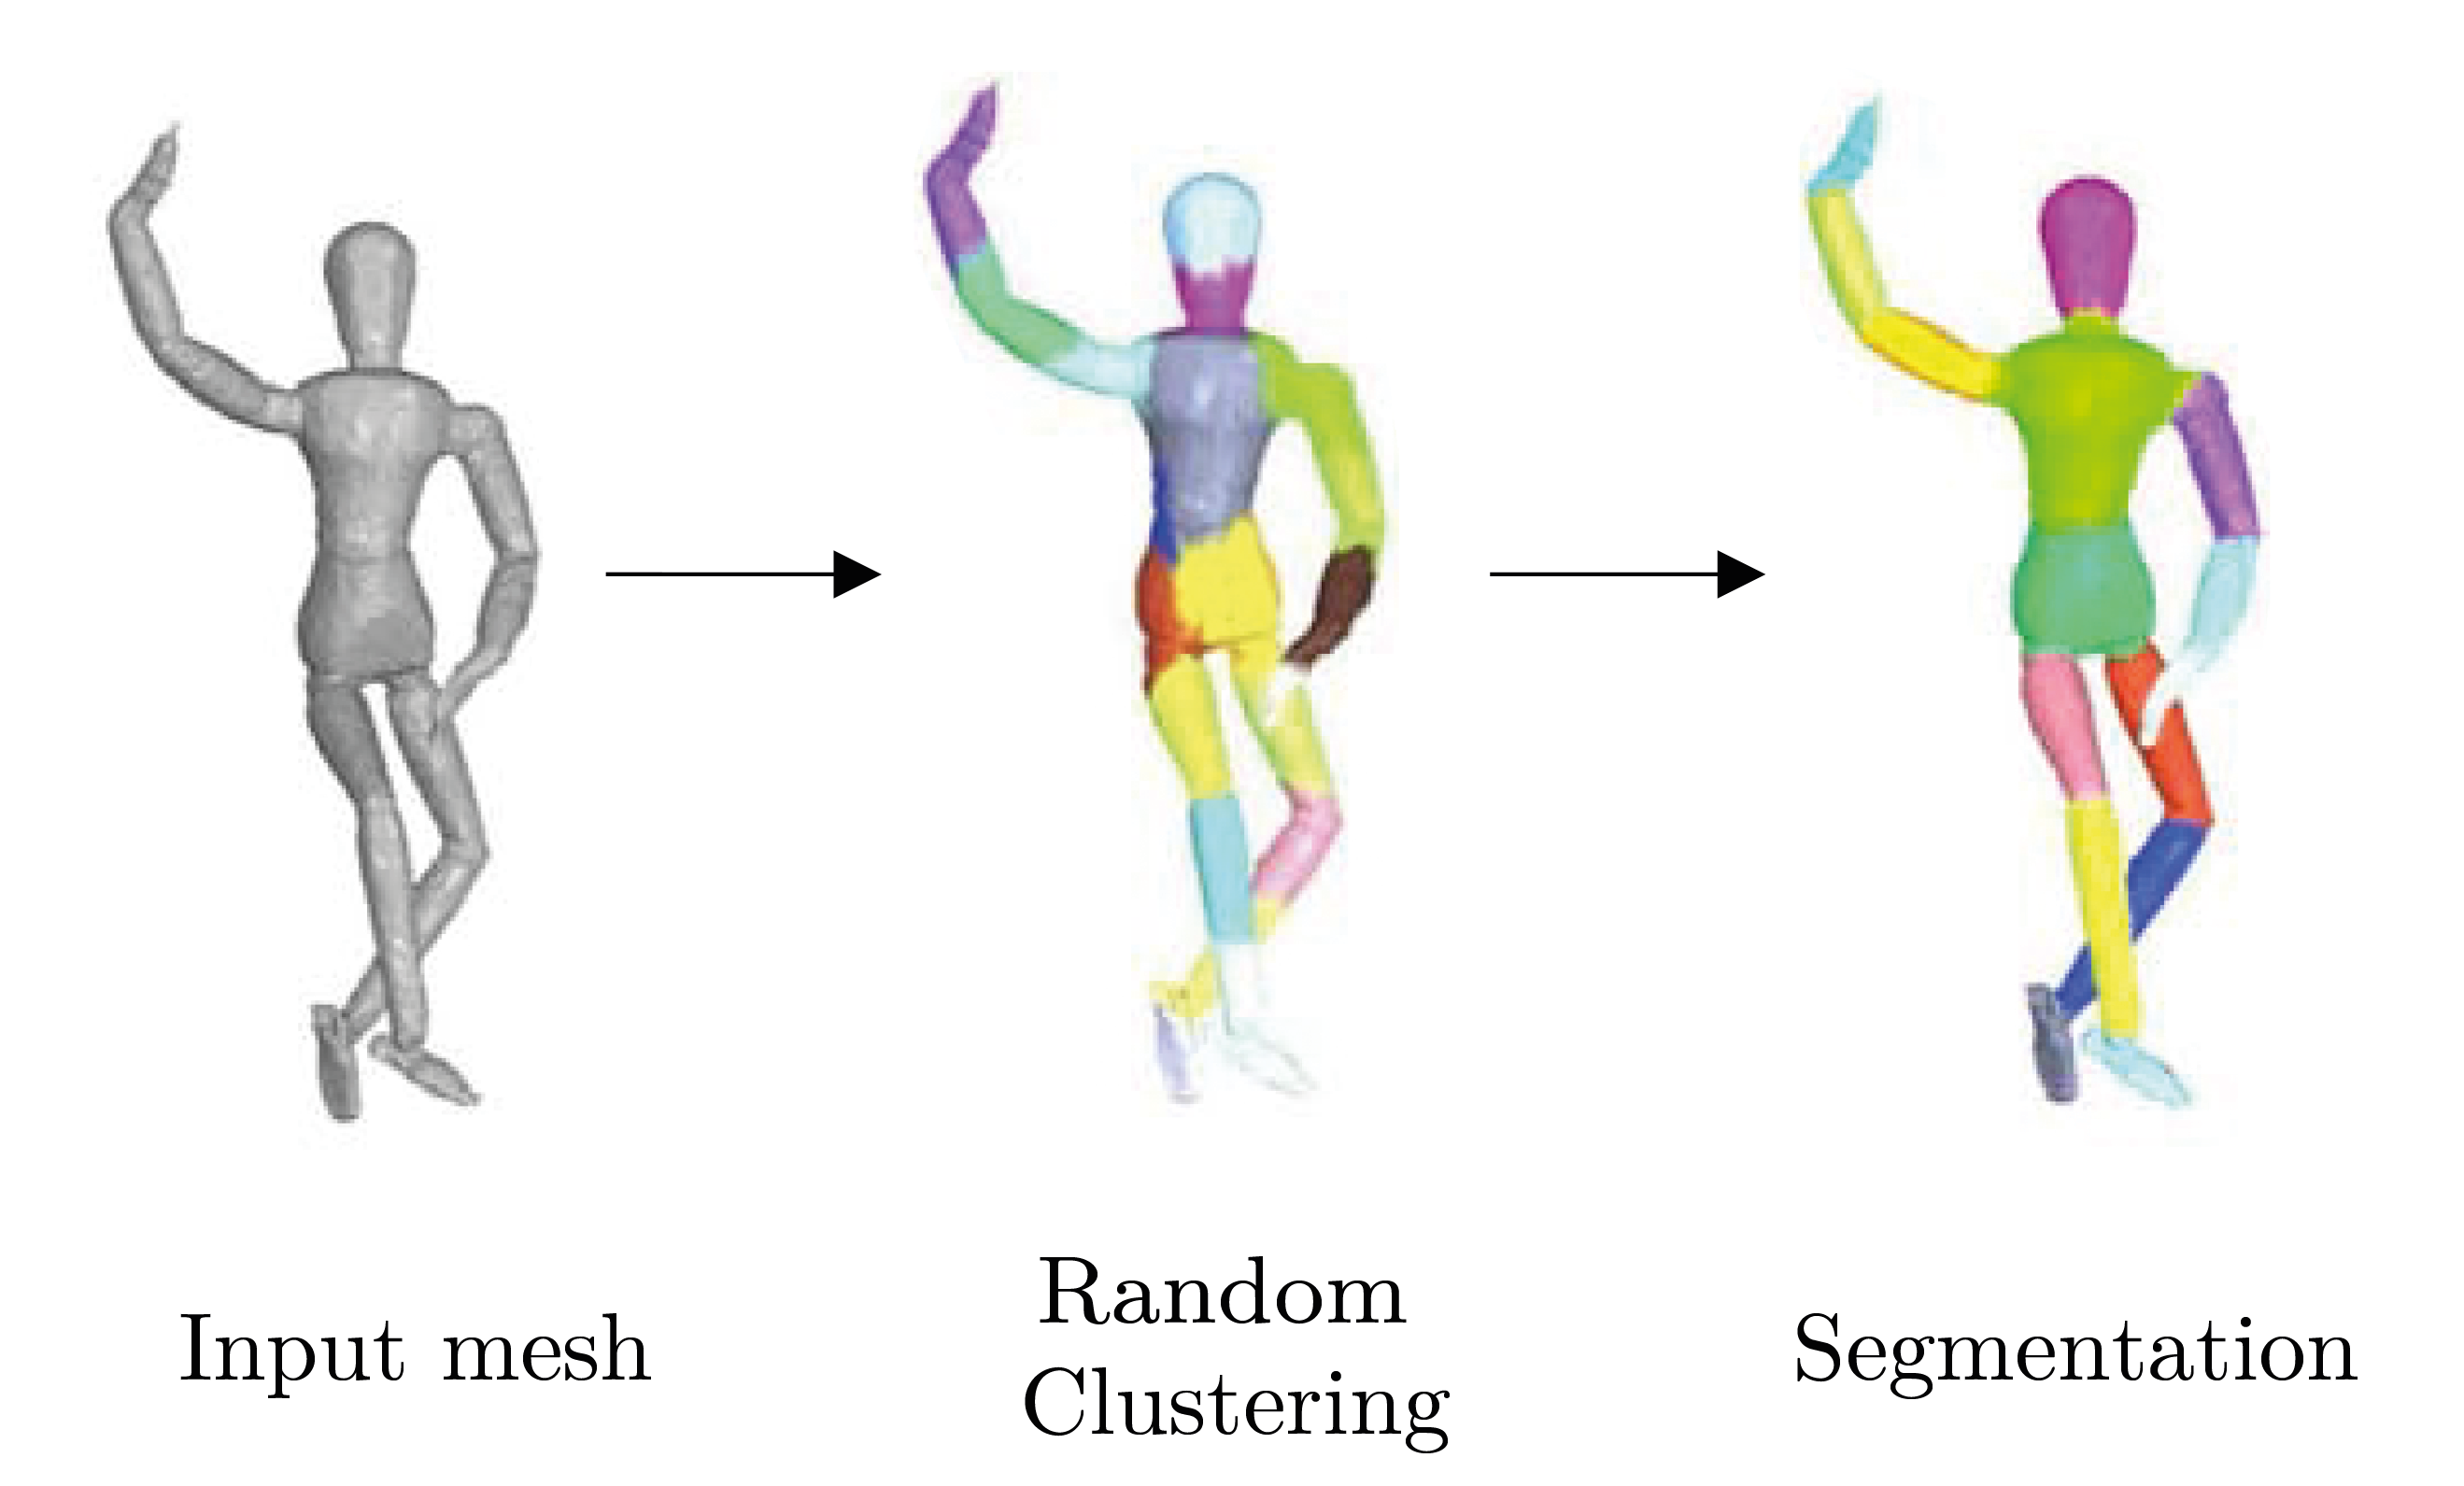
\includegraphics[width=0.7\linewidth]{anguelov}
	\caption{Segmentation a template mesh $M$ into its rigid parts by applying random clustering and a probabilistic framework to iteratively detect associating parts in another mesh \cite{Anguelov04}.}
	\label{fig:correlatedcorrespondance}
\end{figure}
%%
A different approach proposes the recursive detection of body parts by the LRP -- ``largest rigid part'' algorithm \cite {guo2016correspondence}. 
%%
\section{LRP}
The LRP algorithm discovers the articulated parts of two objects in different configurations by initially detecting the largest rigid part. This would be the biggest point cluster by applying a single rigid transformation. To reach that, sparse correspondences in combination with RANSAC are implemented. From there, the linking parts are recursively detected by growing clusters from the LRP and reapplying the algorithm. 
%%
\begin{figure}[H]
	\centering\small
	\begin{tabular}{cc}
		\fbox{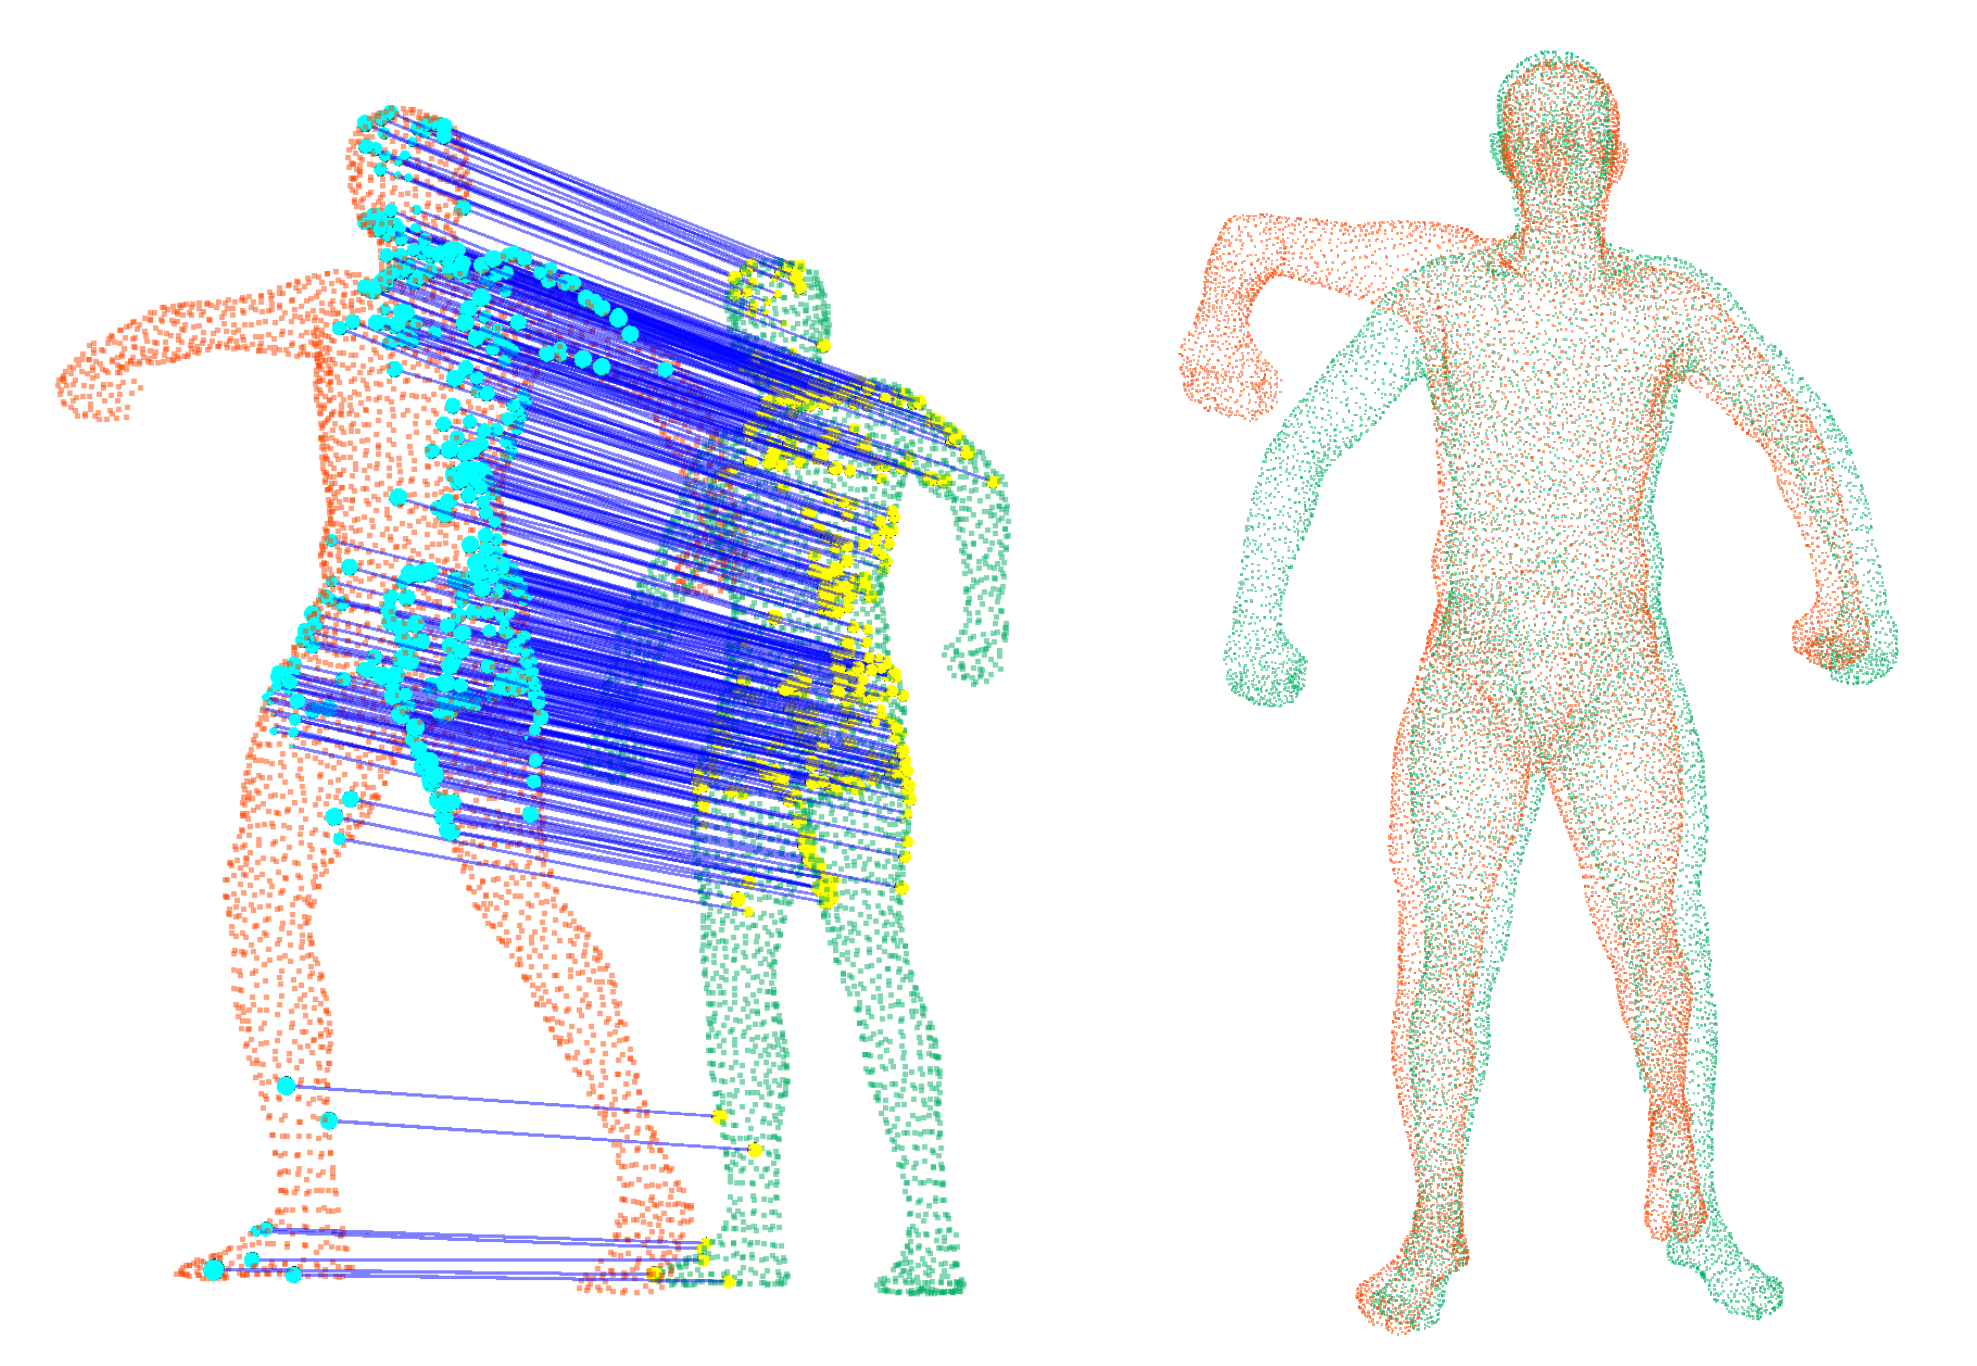
\includegraphics[width=0.45\textwidth]{LRP_body}} &	
		\fbox{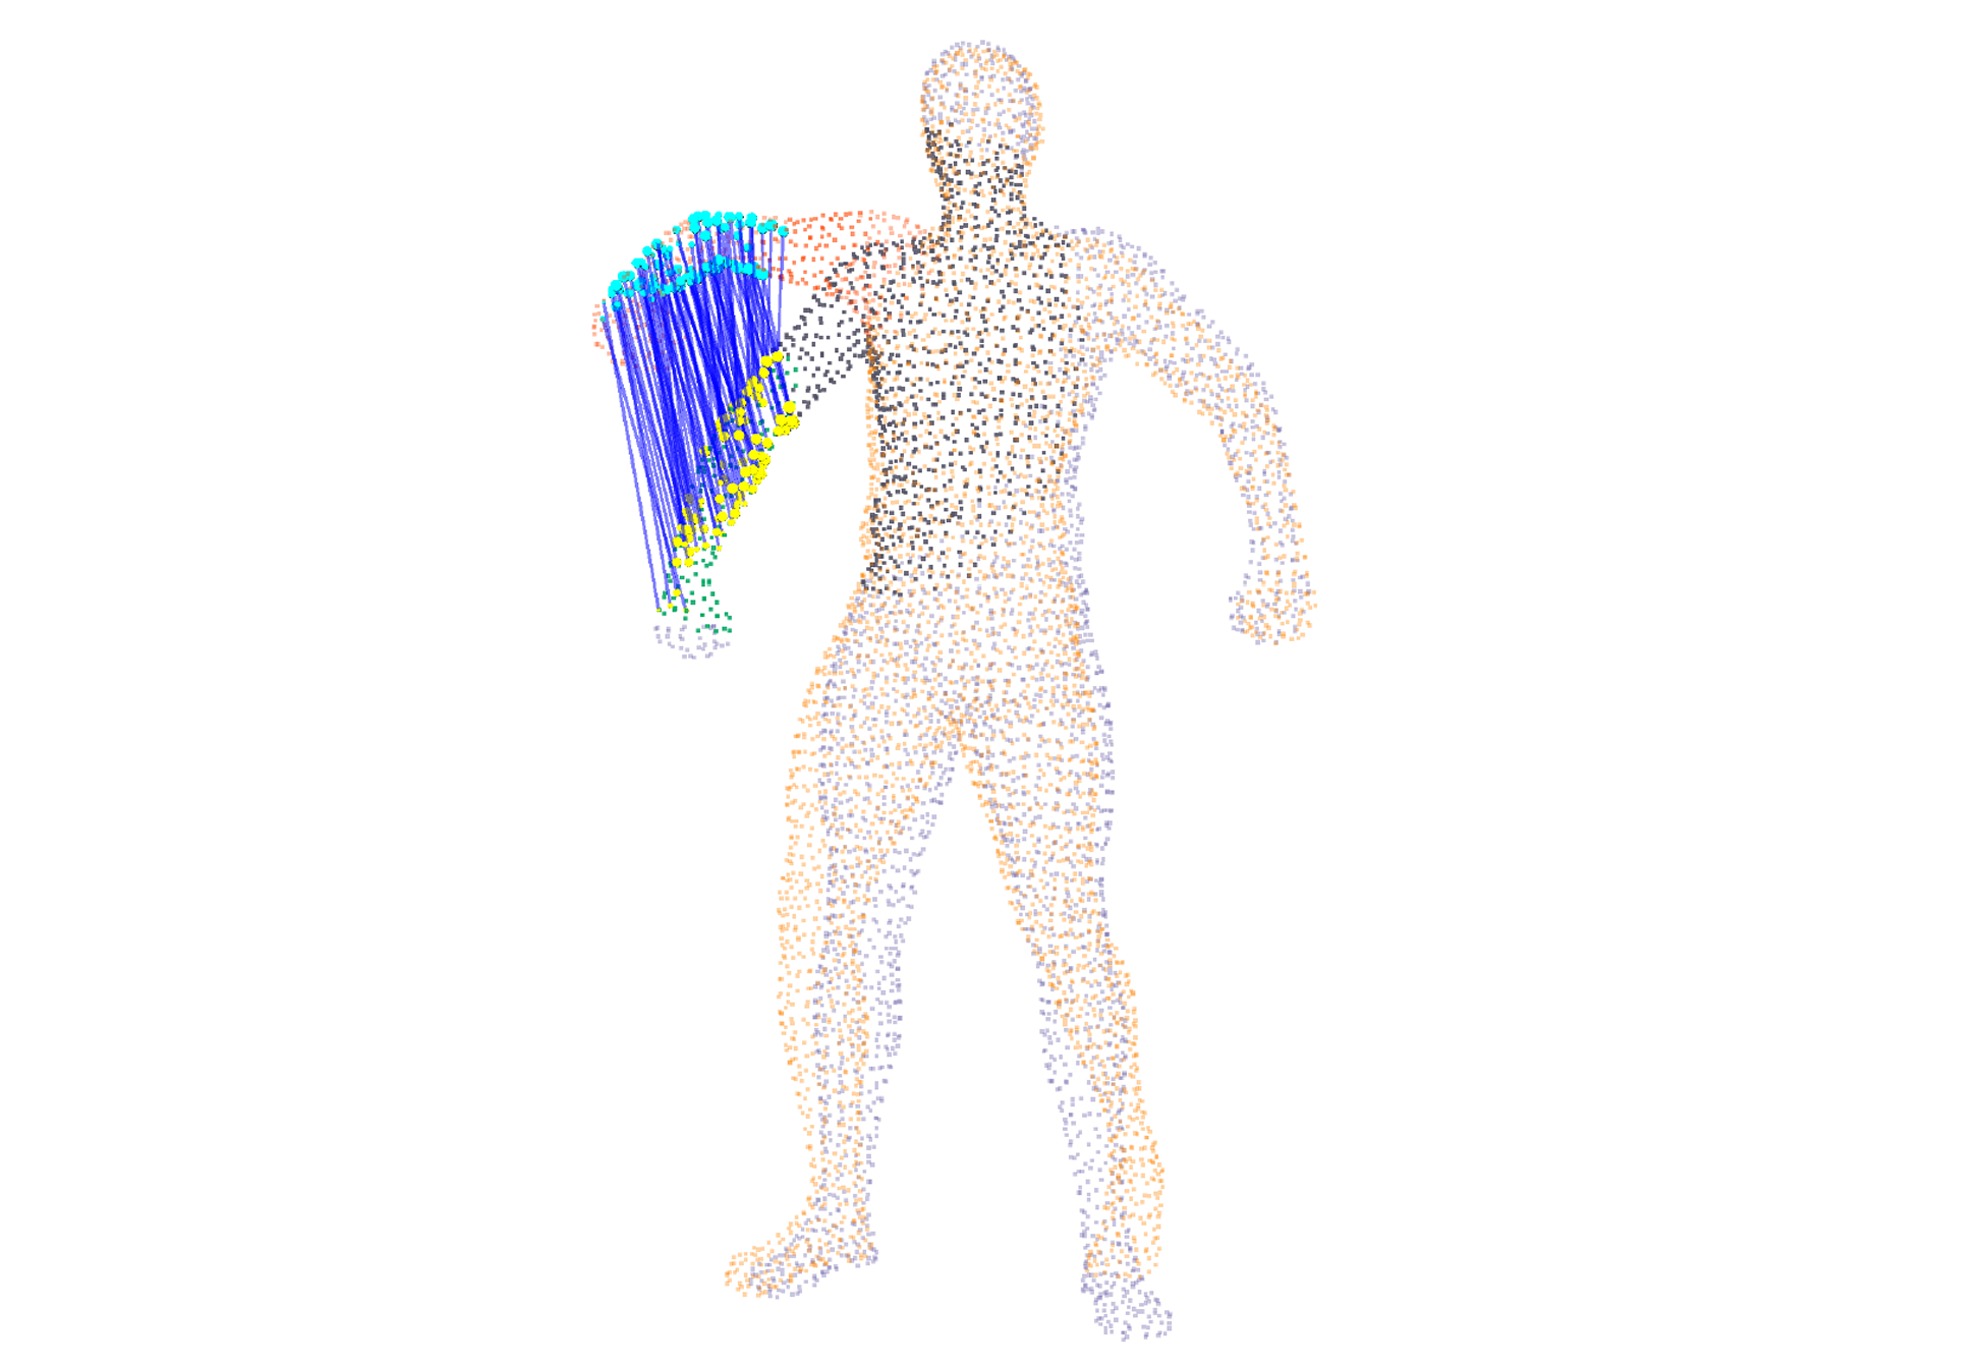
\includegraphics[width=0.45\textwidth]{LRP_arm}} 
		\\
		(a) & (b) 
	\end{tabular}
	\caption{Detecting the largest rigid part of an object~(a), and align the object to recursively detect linking parts to the LRP~(b) \cite{guo2016correspondence}.} 
	\label{fig:LRP_algorithm}
\end{figure}
%%
Another approach is achieved by Symmetrization \cite{Mitra07}, by detecting and aligning the body parts’ symmetry axes of an object(see figure \ref{fig:Symmetrization}). Based on Anguelov \cite{Anguelov04} and Mitra \cite{Mitra07}, Chang et al developed a closely related approach \cite{chang08articulated} \cite{chang09range}.
%%
\begin{figure}[H]
	\centering\small
	\begin{tabular}{cc}
		\fbox{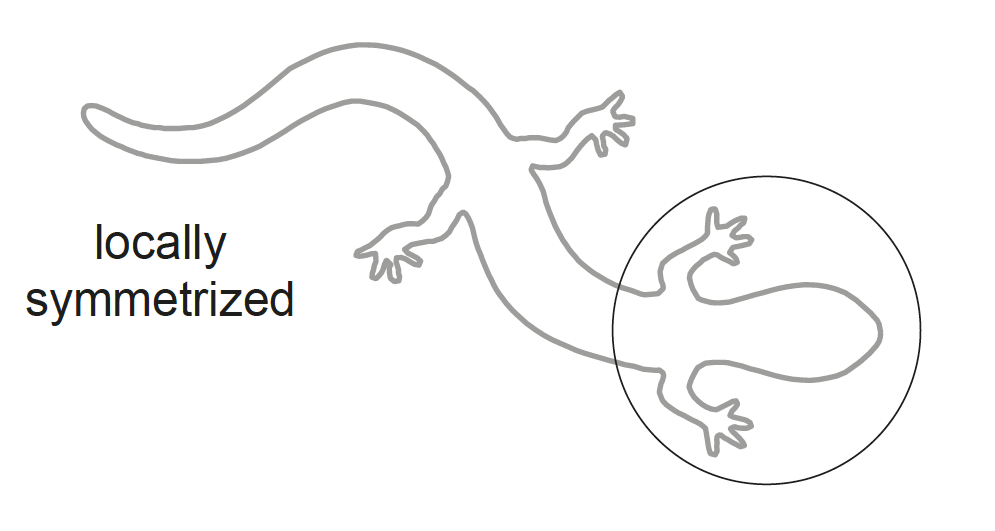
\includegraphics[width=0.45\textwidth]{Symmetrization1}} &
		\fbox{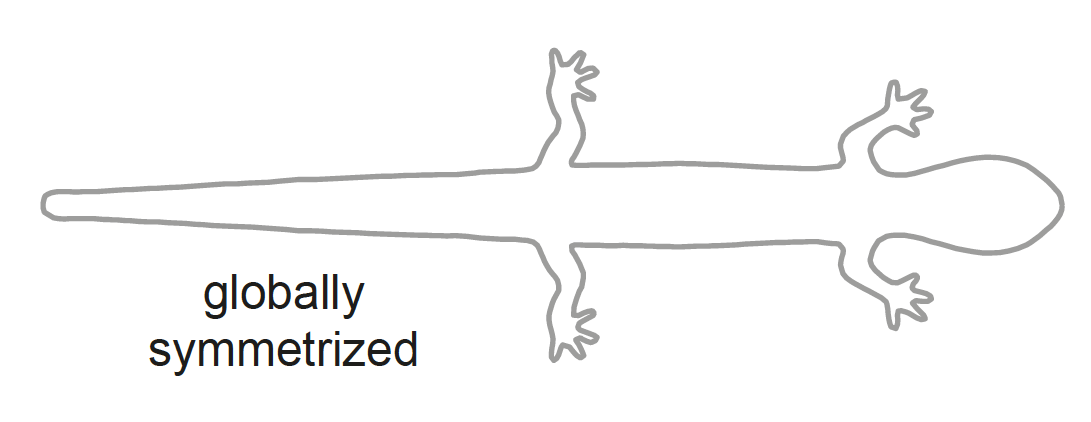
\includegraphics[width=0.45\textwidth]{Symmetrization2}} 
		\\
		(a) & (b) 
	\end{tabular}
	\caption{Detection of the rigid parts of an object by local~(a) and global~(b) Symmetrization \cite{Mitra07}.} 
	\label{fig:Symmetrization}
\end{figure}
%%

%TODO: Add other references
\section{Possible improvements}

%TODO: What are the main deficits of the algorithms?

The proposed approaches achieve convincing results concerning the accuracy of the segmentation and the detection of rigid parts. However, they are all computationally expensive and require a considerable number of computation steps to iteratively detect rigid parts in two associated objects. This reflects on the run time of the algorithm which offers therefore great potential for improvements.
\chapter{Notation}
\label{cha:Notation}

\begin{itemize}
	%use \dotfill for points
	\item[$M$] Input mesh
	\item[$\mathcal{P}$] set of rigid parts
	\item[$\mathcal{J}$] set of joints
	\item[$\mathcal{C}$] set of clusters
	\item[$\mathcal{T}$] set of transformations
	\item[$C_i$] cluster
	\item[$C_{i,j,\cdots}$] sub cluster with varying depth
	\item[$p_i$] principal axis of $C_i$
	\item[$s_i$] secondary axis of $C_i$
	\item[$\theta$] orientation of $C_i$
	\item[$\boldsymbol{p}_i(x,y)$] 2D cluster point of $C_i$
	\item[$\boldsymbol{p}_i(x,y,z)$] 3D cluster point of $C_i$
	\item[$\boldsymbol{c}_i(x,y)$] centroid of $C_i$
	\item[$\boldsymbol{j}_i(x,y)$] joint between two clusters $C_i$ and $C_j$
	\item[$g(\boldsymbol{p}_i,\boldsymbol{p}_j)$] geodesic distance between two cluster points
	\item[$d(\boldsymbol{p}_i,\boldsymbol{p}_j)$] euclidean distance between two cluster points
	\item[$e$] matching error between two clusters
	\item[$e_{avg}$] average matching error between two clusters 
	\item[$e_{PF}$] matching error between two clusters applying Procrustes fitting
	\item[$\tau$] error threshold 
	\item[$N$] Node in a tree
	\item[$\mathit{left}$] left child of $N$
	\item[$\mathit{right}$] right child of $N$
	\item[$\mathcal{L}$] set of final sub cluster pairs
	\item[$L_{i,j}$] sub cluster of $\mathcal{L}$	
	\item[$\mathcal{U}$] set of unclustered points
	\item[$\boldsymbol{u}_i(x,y)$] unclustered point
	\item[$r$] radius
	\item[$\vec{n}$] normal vector
	\item[$H_i$] feature histogram of a point $p_i$
	\item[$H_\mu$] mean feature histogram of a cluster $C_i$
\end{itemize}



\chapter{Initial position}
\label{cha:requirements}

Taking the existing methods as reference (see chapter \ref{cha:RelatedWork}) a new segmentation approach is developed. Thereby, the main focus is to reduce the computation steps of the correlated correspondence algorithm \cite{CorrelatedCorrespondance} as well as the LRP algorithm \cite {guo2016correspondence}. To fully focus on the segmentation into its rigid part, the 3D reconstruction of the articulated object is assumed to be available.

\section{Goal}

The goal is to segment an articulated mesh $M$ into its unknown number $n$ of rigid parts $\mathcal{P} =  \{P_1,\ldots,P_n\}$ and extract all joints $m$ $\mathcal{J} =  \{J_1,\ldots,J_m\}$ linking those parts in form of a skeleton structure. In general, this is done by non-rigid registration of the point clouds $C_1$ and $C_2$ of an object in two different poses. $C_1$ is thereby used as a \textit{template} to be registered with $C_2$. The main task is to determine a part assignment $P_i$ and the corresponding transformation $T_i$ for all points of the \textit{template} that aligns them with all points of $C_2$. Basically, a divide and conquer approach is implemented to recursively subdivide $C_1$ and $C_2$ into matching sub clusters. 

\section{Assumptions}

The input mesh $M$ is assumed to solely consist of rigid parts that can not be deformed or stretched (e.g. rigid parts of a human) and are linked by joints. Comparing two poses being adopted by the articulated object, the geodesic distance $g(\boldsymbol{p}_i,\boldsymbol{p}_j)$ between two mesh points $\boldsymbol{p}_i(x,y)$ and $\boldsymbol{p}_j(x,y)$ remains constant. Thereby, it is taken advantage of the knowledge that points located on a rigid part $P_i$ have the same transformation $T_i$ . Furthermore, it is assumed that the two poses of $M$ are oriented in the same direction.

\section{Chosen environment}

The initial approach was implemented in Java, using ImageJ as processing library. The chosen environment depends on the following factors:
\begin{itemize}
	\item familiarity and prior experience
	\item complexity
	\item available plug-in for image processing
\end{itemize}
%%
As ImageJ is mainly used for 2D use cases, another implementation would be possible in 3D using PCL in C++. As a result, the attention can be brought to segmentation and visualization in 3D.
\chapter{Optimization approach}
\label{cha:TheThesis}

Taking the existing methods as reference (see chapter \ref{RelatedWork}) a new segmentation approach is developed. Thereby, the main focus is to reduce the computation steps of the correlated correspondence algorithm \cite{CorrelatedCorrespondance} as well as the LRP algorithm \cite {guo2016correspondence}. The approach has been first implemented in 2D, in order to be able to focus solely on developing and testing. Subsequently, it will be implemented in 3D using the PCL.

\section{Goal}

The goal is to segment an articulated mesh $M$ into its unknown number $n$ of rigid parts $\mathcal{P} =  \{P_1,\ldots,P_n\}$ and extract the joints $\mathcal{J} =  \{J_1,\ldots,J_m\}$ linking those parts in form of a skeleton structure. In general, this is done by non-rigid registration of the point clouds $C_1$ and $C_2$ of an object in two different poses. $C_1$ is thereby used as a \textit{template} to be registered with $C_2$. The main task is to determine a part assignment $P_i$ and the corresponding transformation $T_i$ for all points of the \textit{template} that aligns them with all points of $C_2$. Basically, a divide and conquer approach is implemented to recursively subdivide $C_1$ and $C_2$ into matching subclusters. 

\section{Assumptions}

The input mesh $M$ is assumed to solely consist of rigid parts that can not be deformed or stretched (e.g. rigid parts of a human) and are linked by joints. Comparing two poses being adopted by the articulated object, the geodesic distance $g(\boldsymbol{p}_i,\boldsymbol{p}_j)$ between two mesh points $\boldsymbol{p}_i(x,y)$ and $\boldsymbol{p}_j(x,y)$ remains constant. Thereby, it is taken advantage of the knowledge that points located on a rigid part $P_i$ have the same transformation $T_i$ . Furthermore, it is assumed that the two poses of $M$ are oriented in the same direction.

\section{General functionality}

The algorithm starts with two sets of point clouds $C_1$ and $C_2$ of an object $M$ in different poses (see figure \ref{fig:pc_2parts}). The two point clouds are iteratively subdivided into point clusters $\mathcal{C}_1 =  (C_{1,1},\ldots, C_{1,m})$ and $\mathcal{C}_2 =  (C_{2,1},\ldots, C_{2,m})$. In each iteration step two related clusters of $C_1$ and $C_2$ are verified to match by applying the ICP (iterative closest point), resulting in a matching error $e$. In case of $ e < \tau $, two clusters are assumed to match. Otherwise, the algorithm is applied recursively and the subclusters are again subdivided. The algorithm terminates if all resulting subclusters of $C_1$ can be matched to all subclusters of $C_2$. Subsequently, they are stored depending on their location and then checked to be merged, in case of having divided a rigid part. After that step, the resulting clusters are assigned to rigid parts $\mathcal{P} =  \{P_1,\ldots,P_n\}$.

\subsection{Removing outliers}

As a first step, the outliers of the point clouds of $M$ are removed. This is done, by iteratively detecting point clusters $\mathcal{C} = \{C_1, \ldots , C_m\}$ from all points of $M$. A cluster $C_i$ is grown from an unclustered point $\boldsymbol{p}_i(x,y)$. Another point $\boldsymbol{p}_j(x,y)$ is added to the cluster $C_i$ if the euclidean distance between them $d(\boldsymbol{p}_i, \boldsymbol{p}_j)$ is below a pre-defined threshold $\tau$. This threshold is thereby depending on the resolution and density of $M$. All points of $C_i$ are then iteratively compared to the remaining unclustered points to allow the cluster to grow. Once, all points of $C_i$ have been treated, another unclustered point is used as a seed. If there are no unclustered points left, the clusters with the highest number of points $n$ are selected as input clusters $C_1$ and $C_2$ (see figure \ref{fig:pc_2parts}).
%%
% TODO: picture of removing outliers
%%
\begin{figure}[htbp]
	\centering\small
	\begin{tabular}{cc}
		\fbox{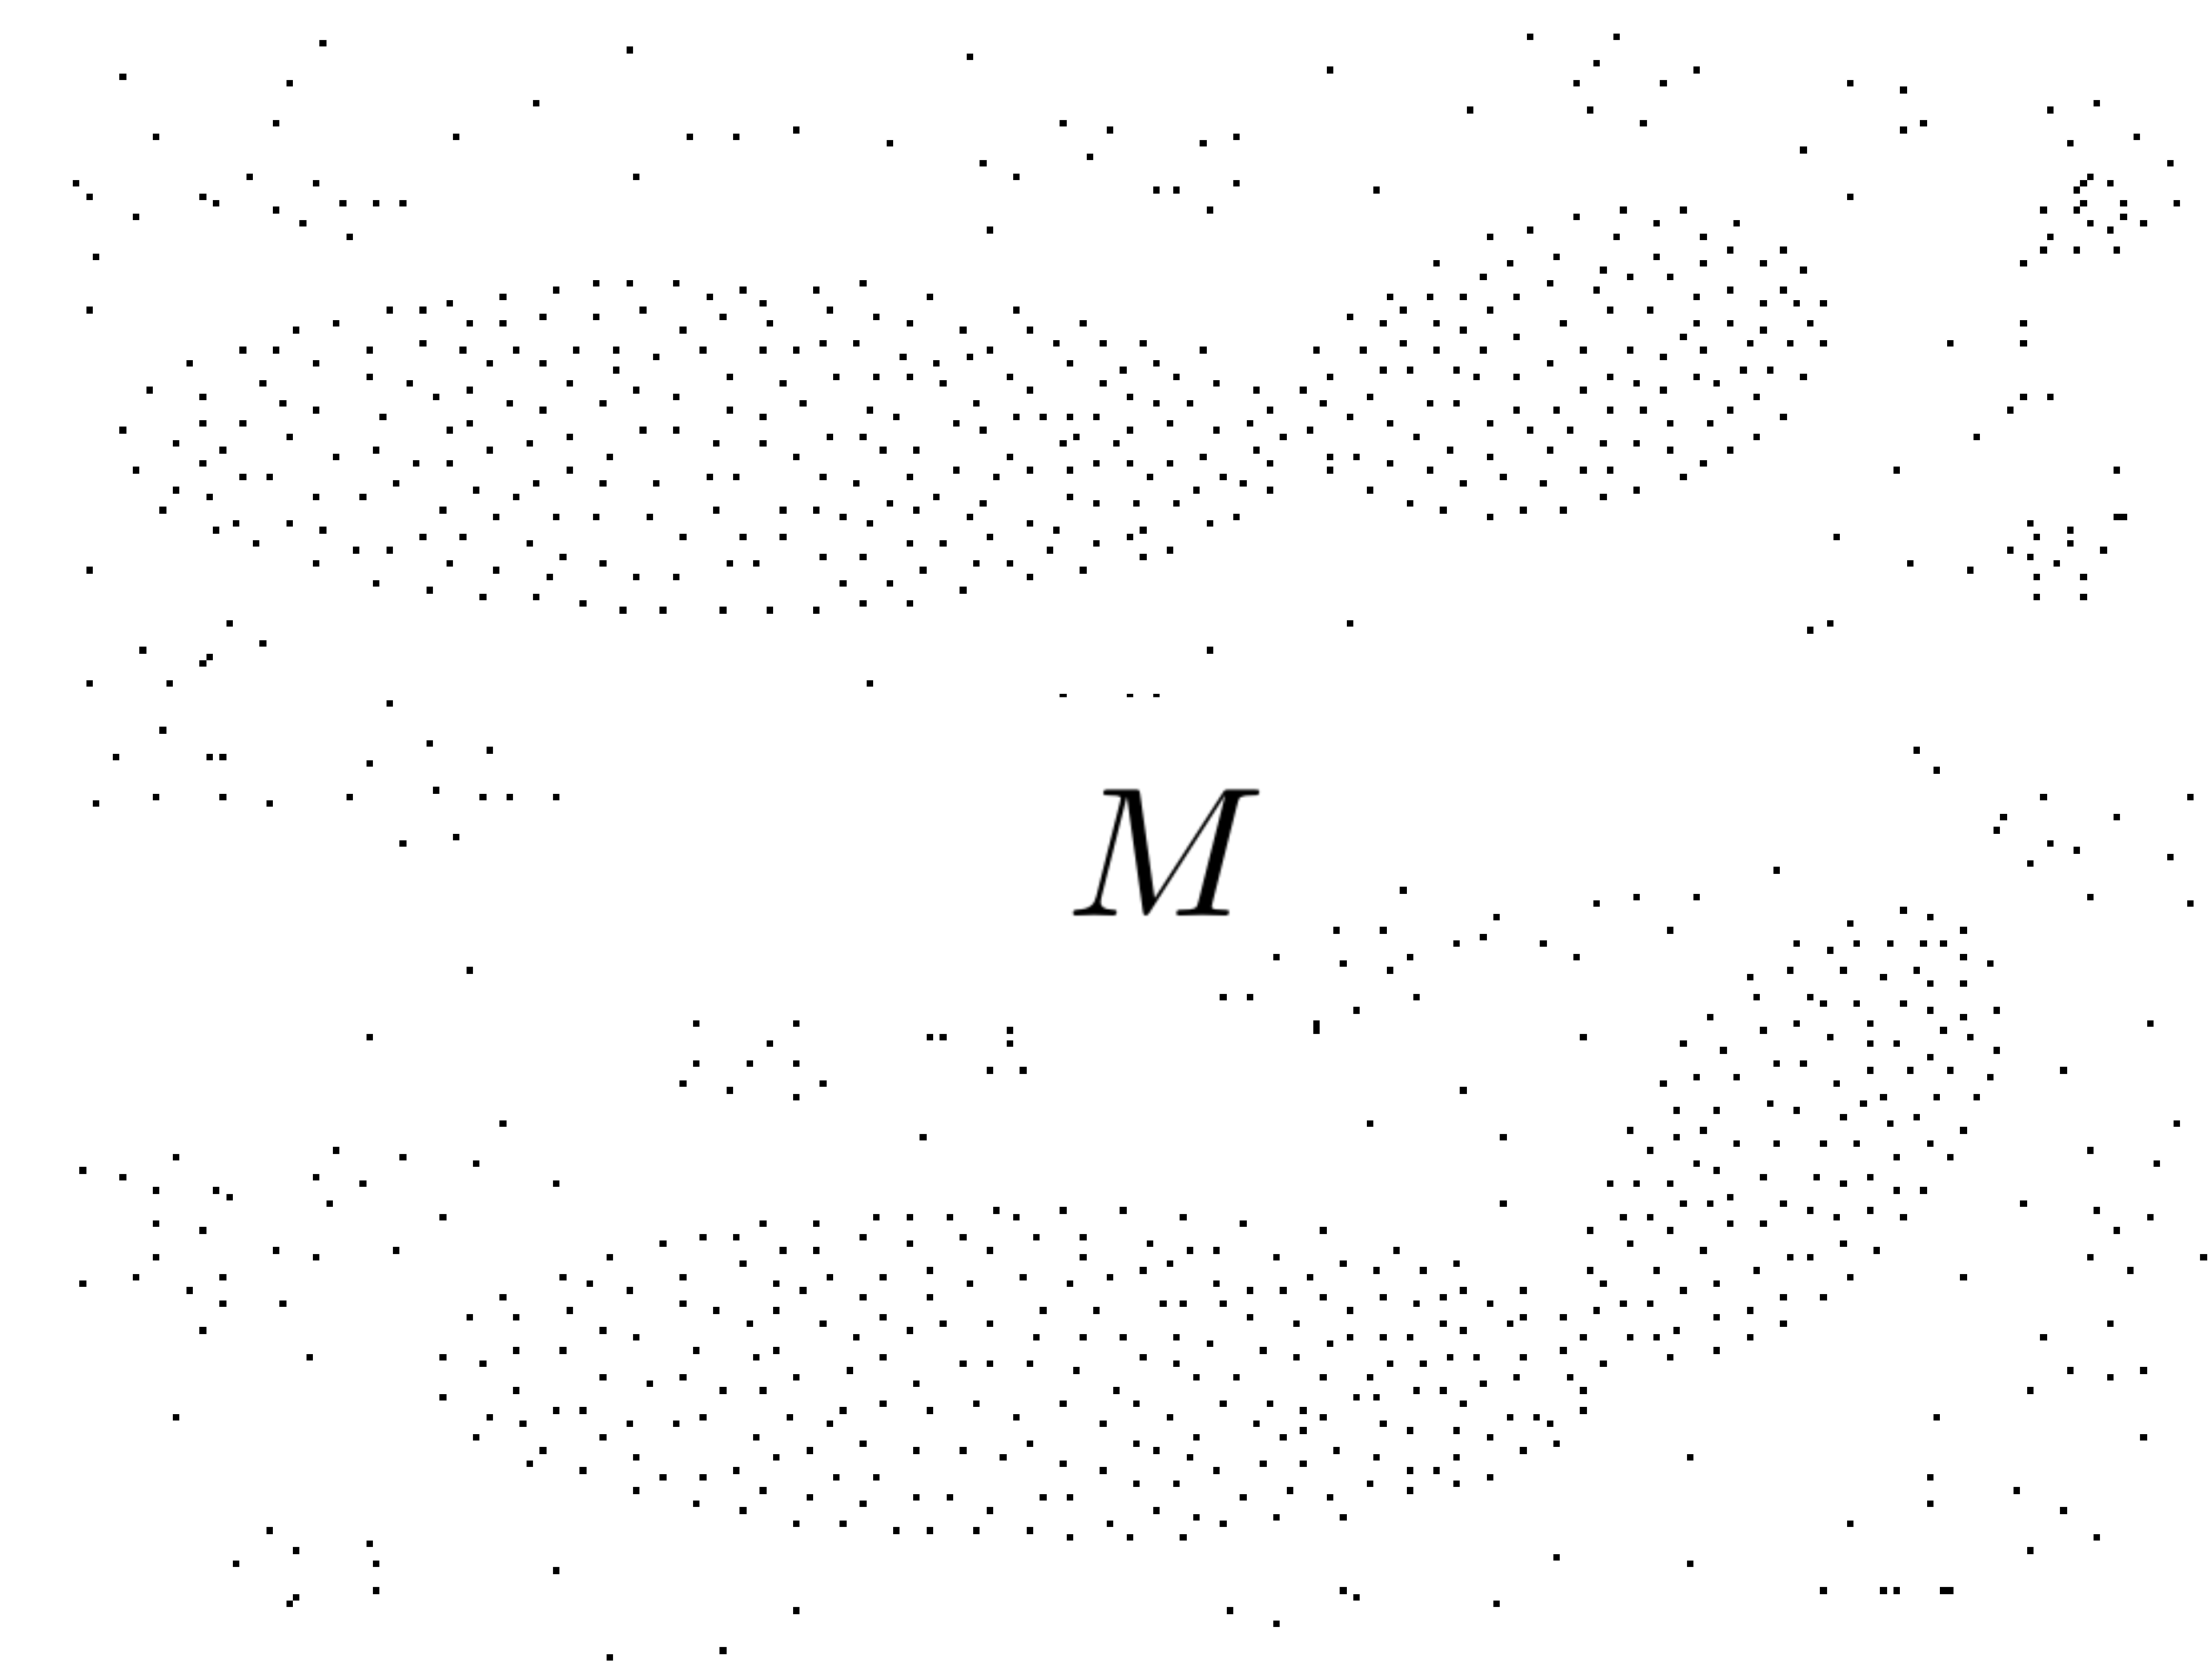
\includegraphics[width=0.45\textwidth]{pc_2parts_Noise}} &		% JPEG file
		\fbox{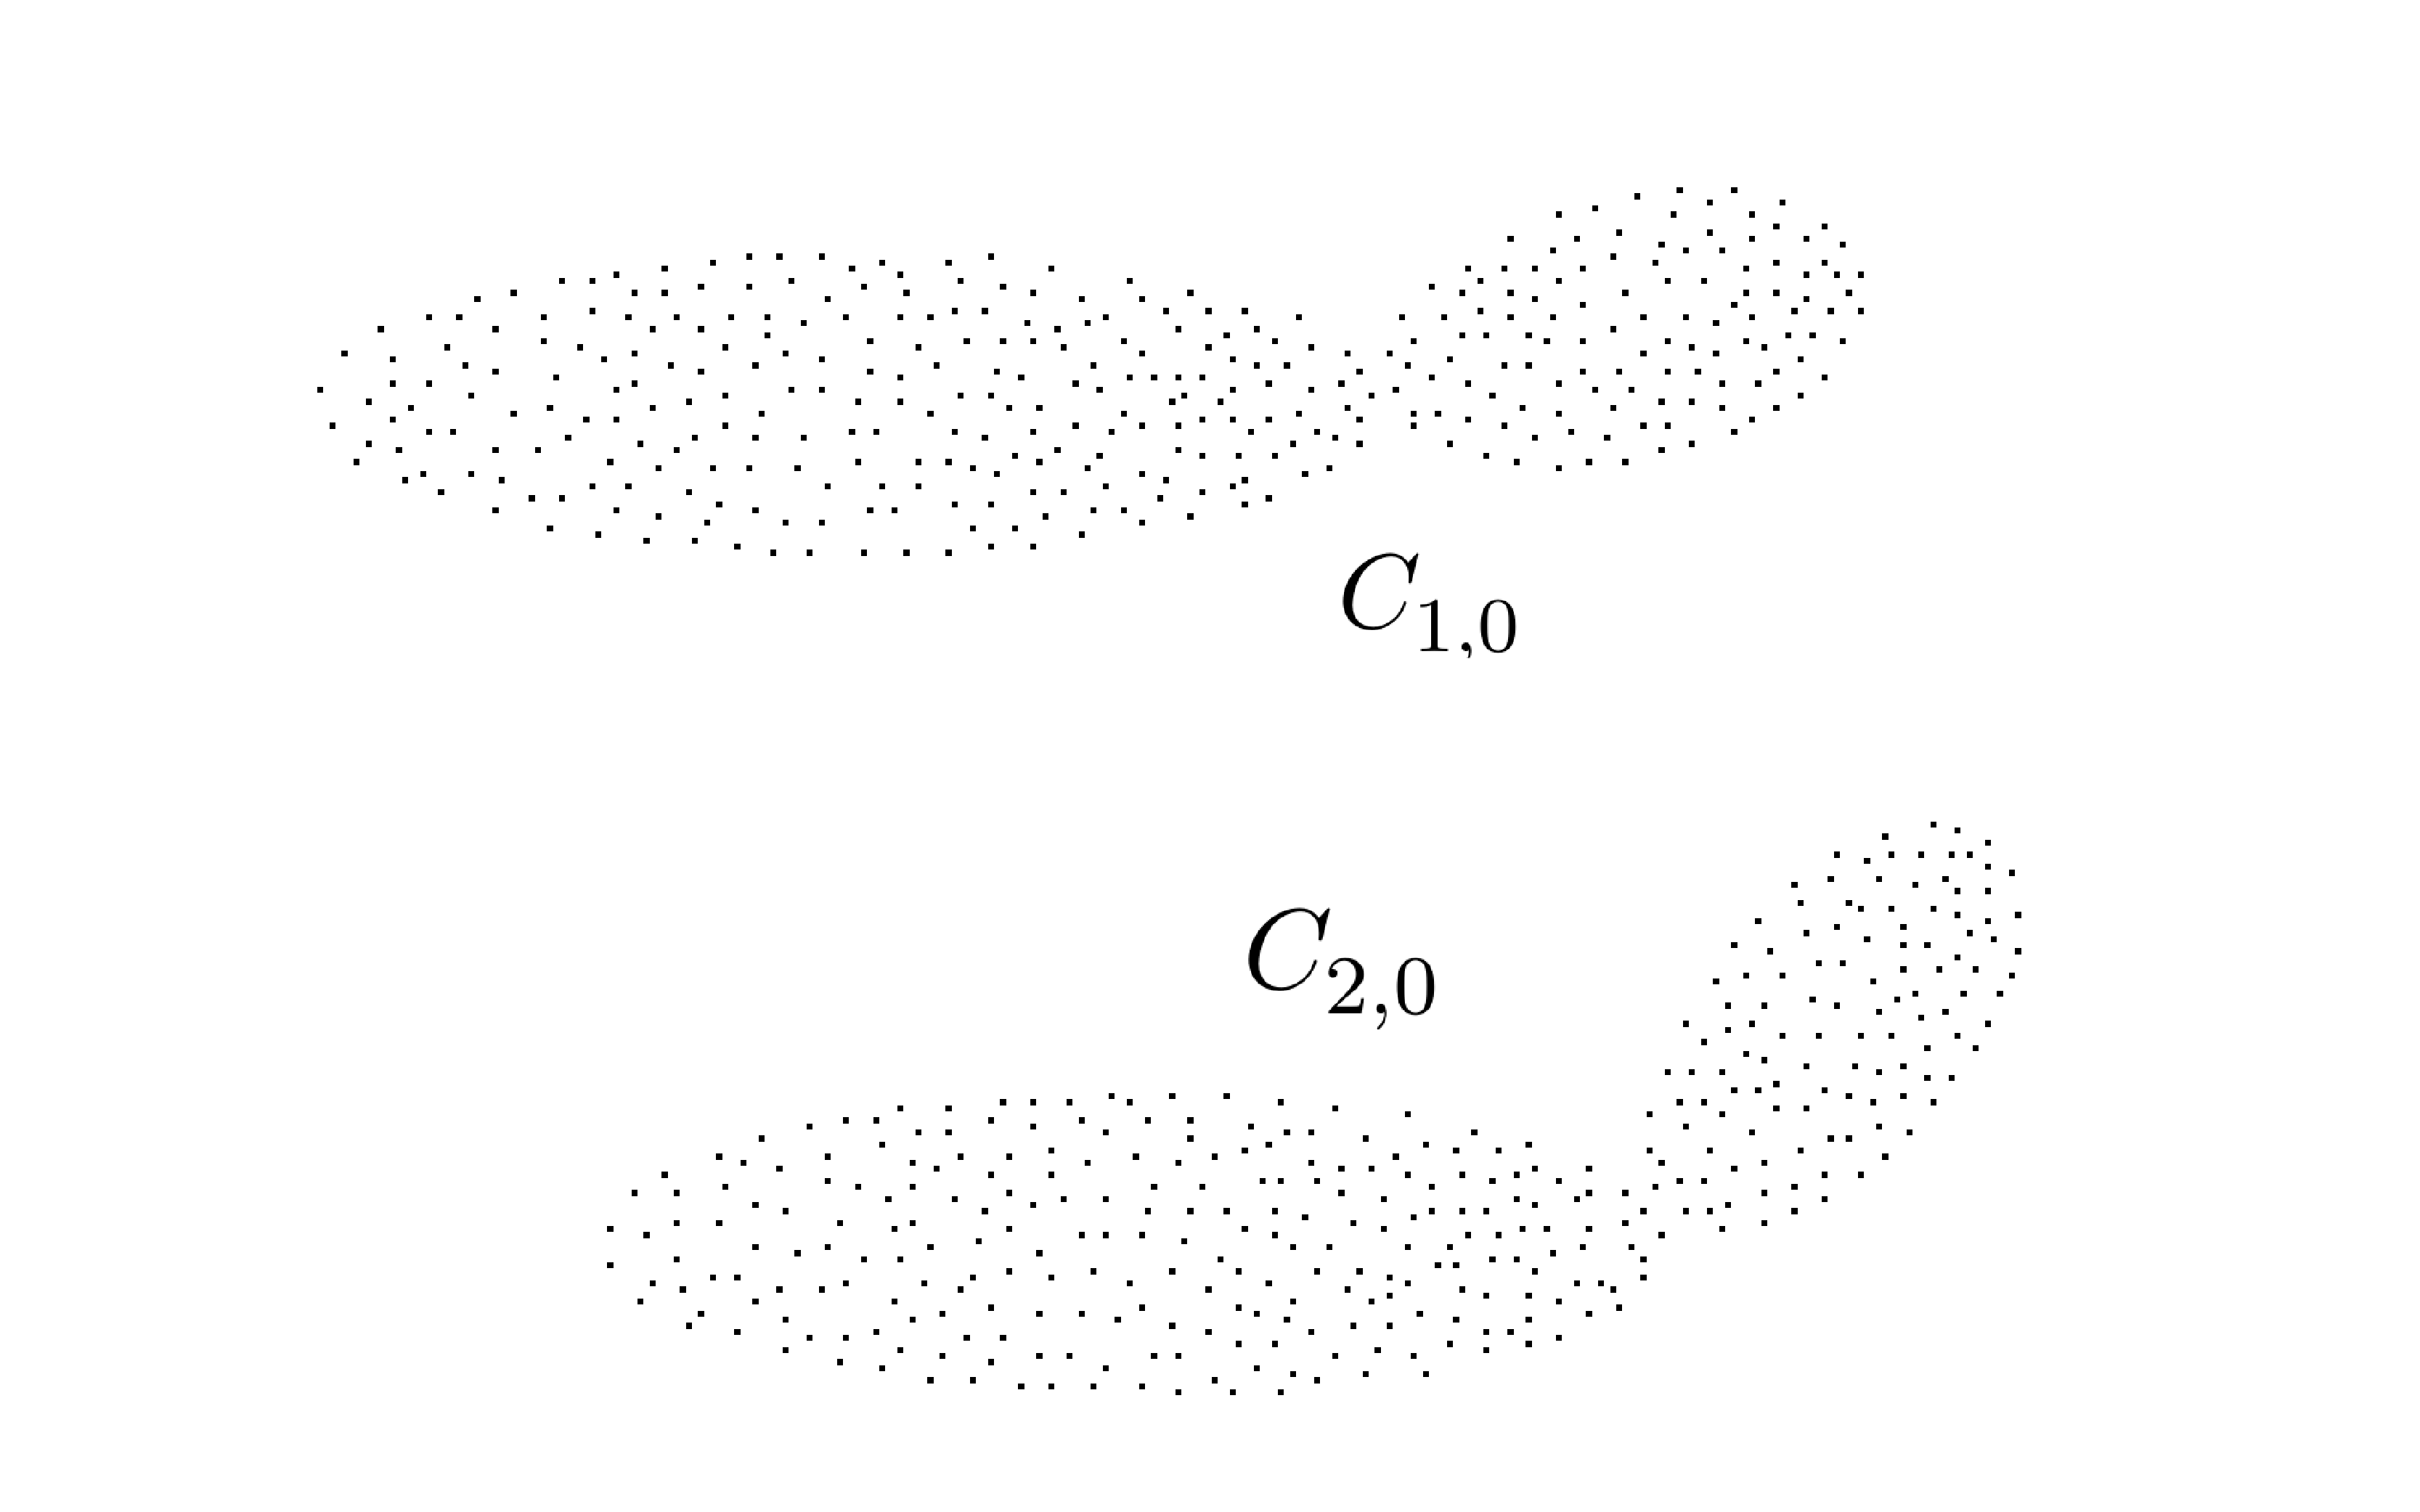
\includegraphics[width=0.45\textwidth]{pc_2parts_noNoise}} 
		\\	% PNG file
		(a) & (b) 
	\end{tabular}
	\caption{Taking a mesh $M$ in two different poses as input (a), removing noise of the input point clouds (b) to achieve the input clusters $C_1$ and $C_2$.} 
	\label{fig:pc_2parts}
\end{figure}

\subsection{Subdividing into clusters}
\label{Subdividing}

As a next step, the two main clusters $C_1$ and $C_2$ are taken as input for further computation steps. If the matching between two clusters does not succeed, they are both subdivided into two sub clusters. Otherwise, no subdividing is done. The whole procedure is repeated recursively for all clusters $\mathcal{C} = (C_{i,1}, \ldots, C_{i,m})$ of $C_1$ and $C_2$ until all associated clusters of $C_1$ match the clusters of $C_2$.  

\subsubsection{Divider position}

To determine where to divide a cluster, it is taken advantage of the principal component analysis (PCA). As a first step, the orientation $\theta$ of $C_1$ and $C_2$ are computed by calculating the central moments
%%
\begin{equation}
	\mu_{pq}(\mathcal{R}) = \sum_{(u,v)\in\mathcal{R}} (u - \bar{x})^p \cdot (v - \bar{y})^q
\end{equation}
%%
\begin{equation}
	\theta(\mathcal{R}) = \frac{1}{2} \tan^{-1} \left(\frac{2\cdot \mu_{11}(\mathcal{R})}{\mu_{20}(\mathcal{R}) - \mu_{02}(\mathcal{R})}\right)
\end{equation}
%%
for each cluster.	
The divider positions are determined by computing the principal axes $p_{1}$ and $p_{2}$ and subsequently taking the perpendicular secondary axes $s_{1}$ and $s_{2}$ through the centroids (see figure \ref{fig:dc_axes_2p}). The secondary axes divide $C_1$ and $C_2$ into the sub clusters $C_{1,1}$ and $C_{1,2}$ as well as $C_{2,1}$ and $C_{2,2}$.

\begin{figure}
	\centering
	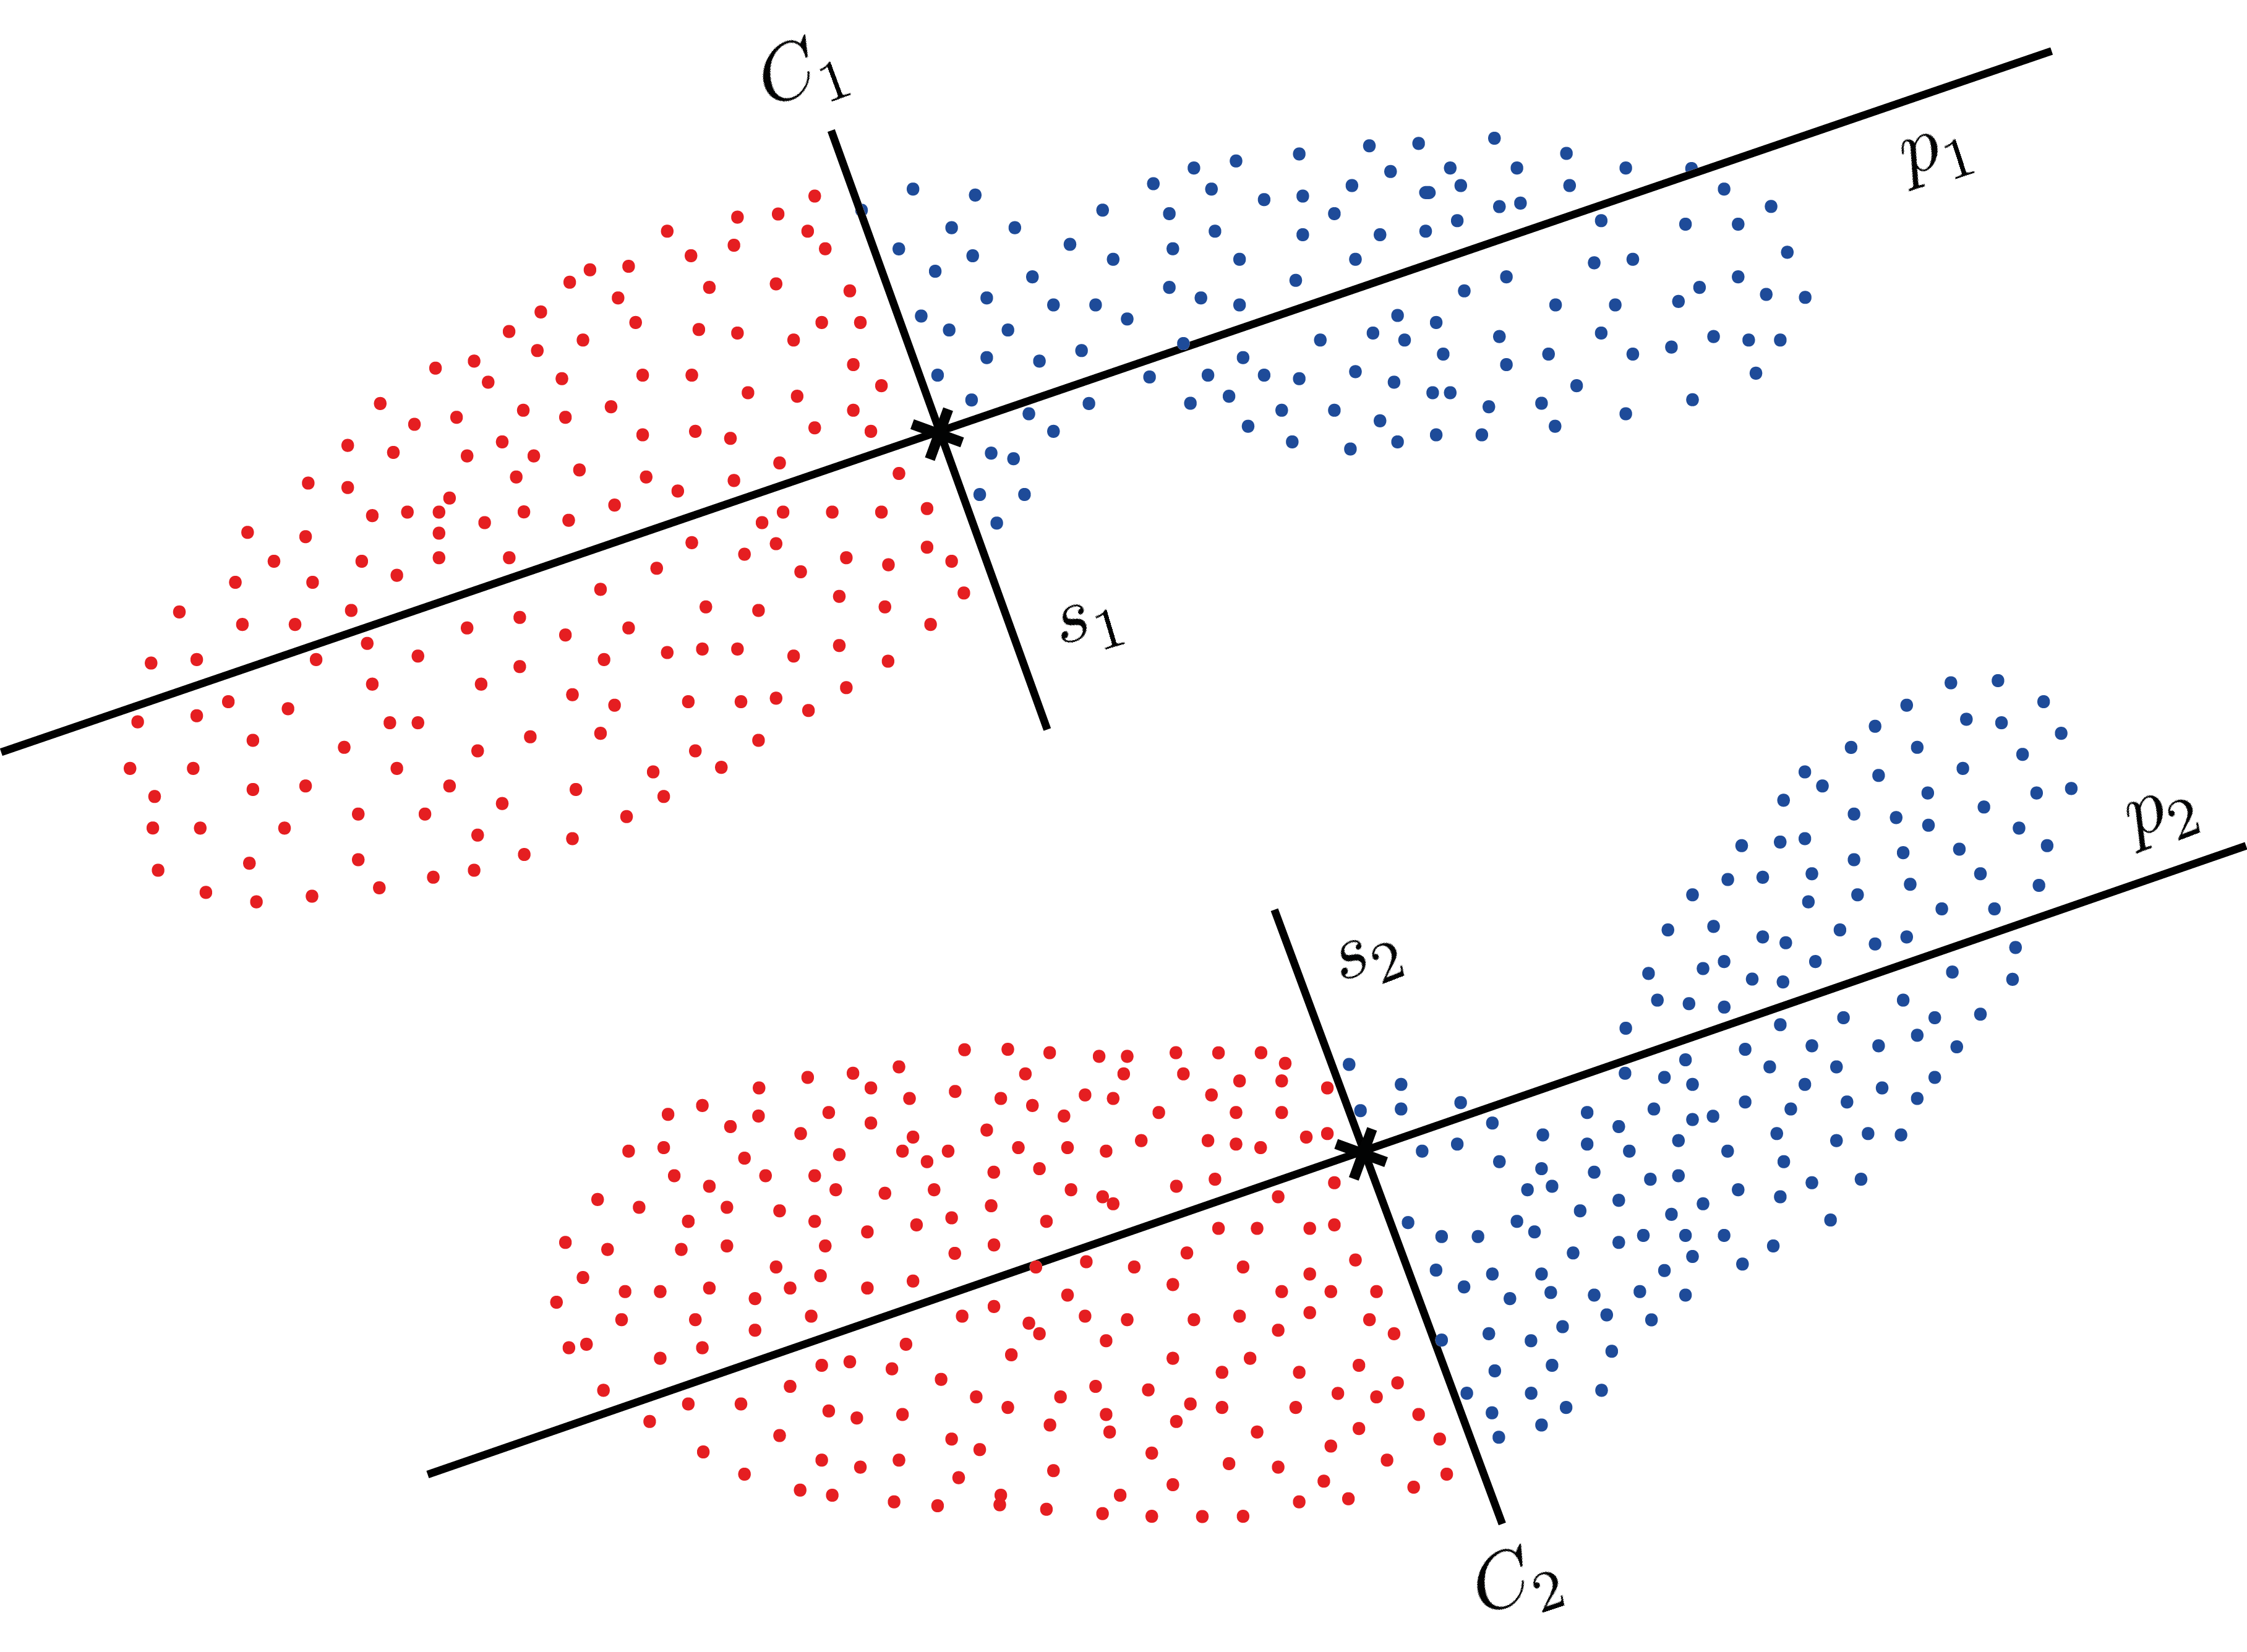
\includegraphics[width=0.8\linewidth]{illustration_axes}
	\caption{Subdividing $C_1$ and $C_2$ into two sub clusters by computing the secondary axes $s_1$ and $s_2$ perpendicular to $p_1$ and $p_2$ through the centroids.}
	\label{fig:dc_axes_2p}
\end{figure}

\subsubsection{Declaring the matching condition between two clusters}

By applying the ICP and the nearest neighbor approach on two associated clusters $C_1$ and $C_2$, a certain matching error $e$ is computed between their cluster points $ C_p =  \{ p_1, \ldots, p_m\}$ and the associated points $ C_q =  \{ q_1, \ldots, q_m\}$. To eliminate the dependency between the matching error and the number of cluster points $m$, the average error per point of $C_p$ and $C_q$
%
\begin{equation}
	e_{\mathrm{avg}(C_p, C_q)} = \frac{1}{| C_p |} \cdot \displaystyle\sum_{i=0}^{m}\| \boldsymbol{p}_i - \boldsymbol{q}_i\|^2
\end{equation}
%
is computed, assuming that the two clusters $C_p$ and $C_q$ contain the same number of cluster points $m$. In case of varying point amounts, the segmentation needs to be carried out differently that subclusters contain the same number of points. Alternatively, extra points are not considered in the error amount calculation. To declare when two clusters match, it is quite essential to determine an appropriate threshold $\tau$ for the maximum distance $d(p_0, q_0)$ between two associated points $p_0$ and $q_0$. In case of being overvalued, clusters are more likely to match which could result in insufficient subdividing. On the other hand, the clusters are difficult to be matched, which will result in further subdividing and the detection of too many rigid parts. The two clusters $C_p$ and $C_q$ are matching, if $e_{avg} < \tau$.

\subsubsection{Cluster tree}
\label{tree}

The subdividing of the clusters $C_1$ and $C_2$ is realized by a depth-first approach in a tree. Consequently, $C_1$ and $C_2$ represent the root and are subdivided from the left to the right. A node $N$ of the tree contains two related clusters $C_{1,i}$ and $C_{2,i}$, where $i$ defines whether the node is a left ($i=1$) or right ($i=2$) node of the parent. In case of further subdividing, a Node $left$, containing the  clusters $C_{1,i,1}$ and $C_{2,i,1}$, as well as a Node $right$, containing the clusters $C_{1,i,2}$ and $C_{2,i,2}$ origin. If two associated clusters $C_{1,i,j}$ and $C_{2,i,j}$ in a Node $N_i$ match, no further subdividing is performed. The resulting leaves of the tree are the final matching sub clusters and stored from left to right in a list $\mathcal{L} = (L_{1,1},L_{2,1},\ldots,L_{1,m},L_{2,m})$ (see figure \ref{fig:illustrationTree}). By applying the depth-first approach, the neighboring clusters in the list are also neighboring clusters in the main clusters $C_1$ and $C_2$.  As a result, in the following step the adjacent sub clusters of $C_1$ or $C_2$ can be merged (see subsection \ref{mergingClusters}).
\begin{figure}
	\centering
	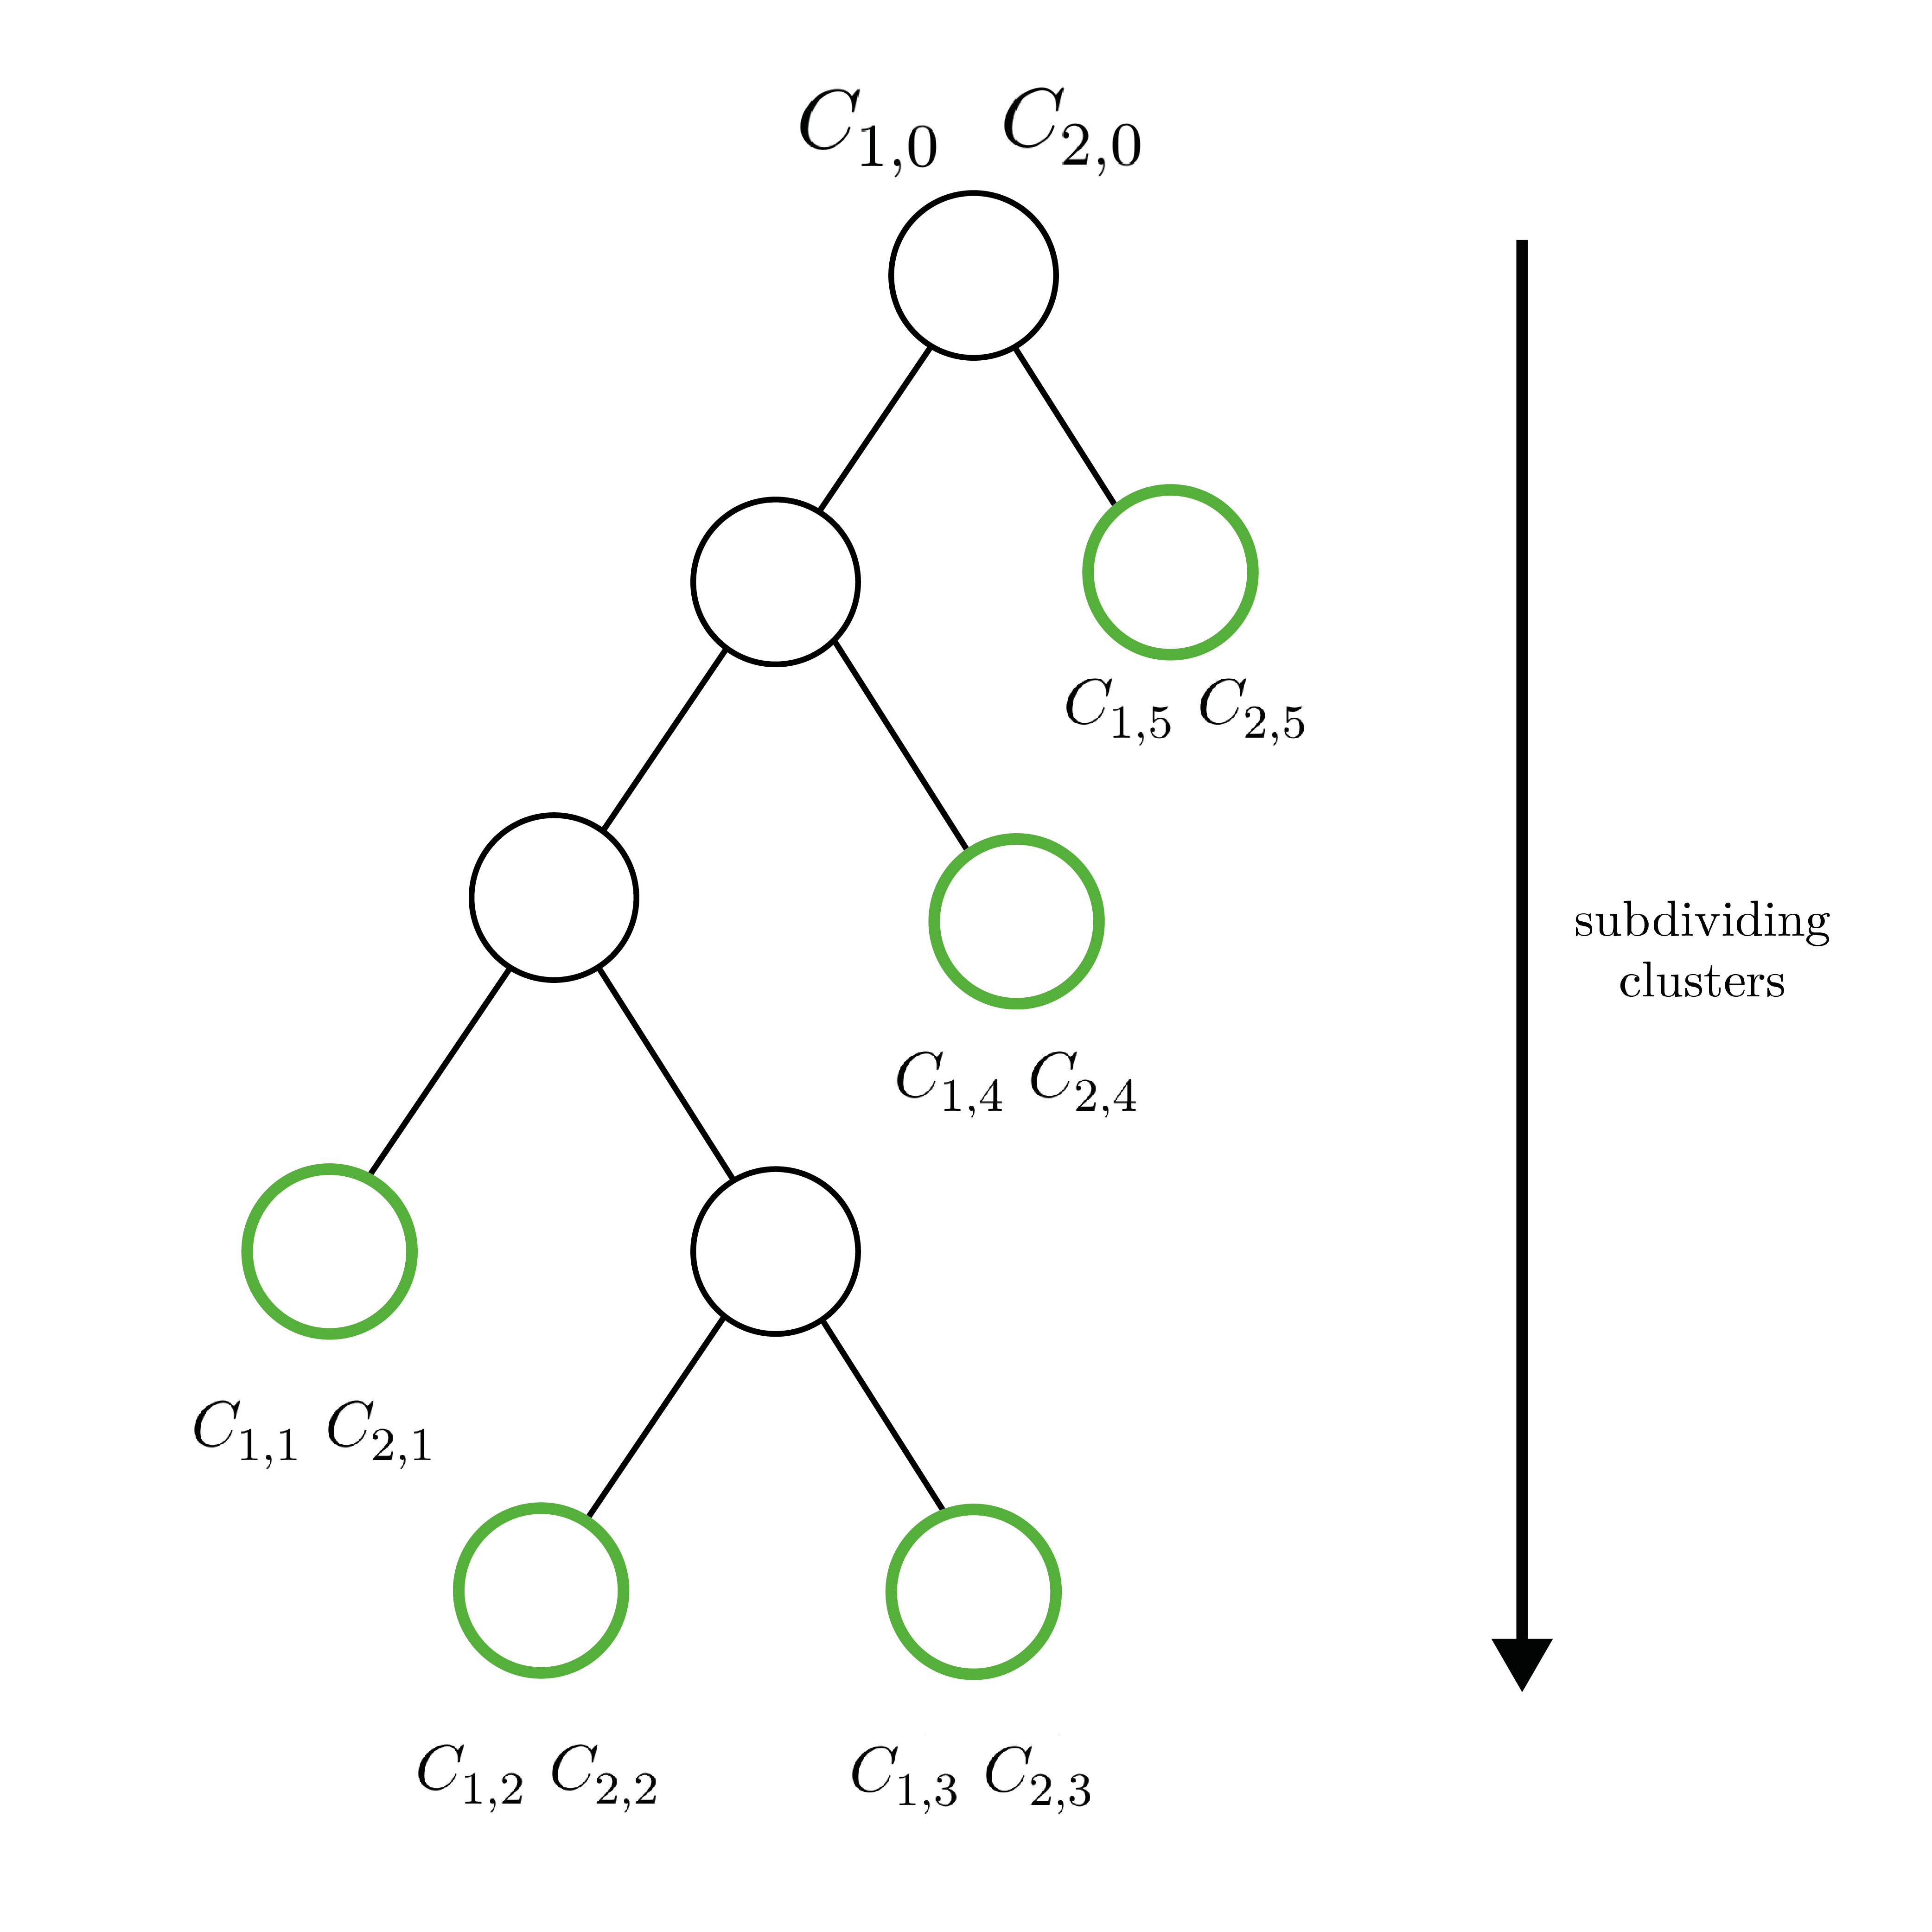
\includegraphics[width=0.7\linewidth]{IllustrationTree}
	\caption{Subdividing of $C_1$ and $C_2$ into matching clusters by a depth-first approach in a tree. The Subdividing terminates if all sub clusters of $C_1$ and $C_2$ match when applying the ICP.}
	\label{fig:illustrationTree}
\end{figure}

\subsection{Merging neighboring clusters to rigid parts}
\label{mergingClusters}
%%
%TODO: Think about renaming!
%%
As a next step, adjacent sub clusters from $\mathcal{L}$ are iteratively merged and subsequently verified to still match. This process is required to rejoin, if necessary, detected sub clusters to the rigid parts of the object. This is the case, if a rigid part was subdivided during the subdividing process (see section \ref{Subdividing}). The merging initiates with the first clusters in the list $L_{1,i}$, $L_{2,i}$ and its adjacent clusters $L_{1,i+1},L_{2,i+1}$. If the resulting merged clusters can be matched, the merging proceeds with the adjacent cluster $L_{1,i+2},C_{2,i+2}$. If not, the merging is not executed and $L_{1,i}$, $L_{2,i}$ are stored in a list of resulting clusters $\mathcal{R}$. The merging procedure then initiates with $L_{1,i+1},L_{2,i+1}$. The process terminates if all clusters of $\mathcal{L}$ are verified and consequently the clusters of $\mathcal{R}$ are assigned to rigid parts $ \mathcal{P} =  \{P_1,\ldots,P_m\}$ (see figure \ref{fig:clusterChain}). 

\begin{figure}
	\centering
	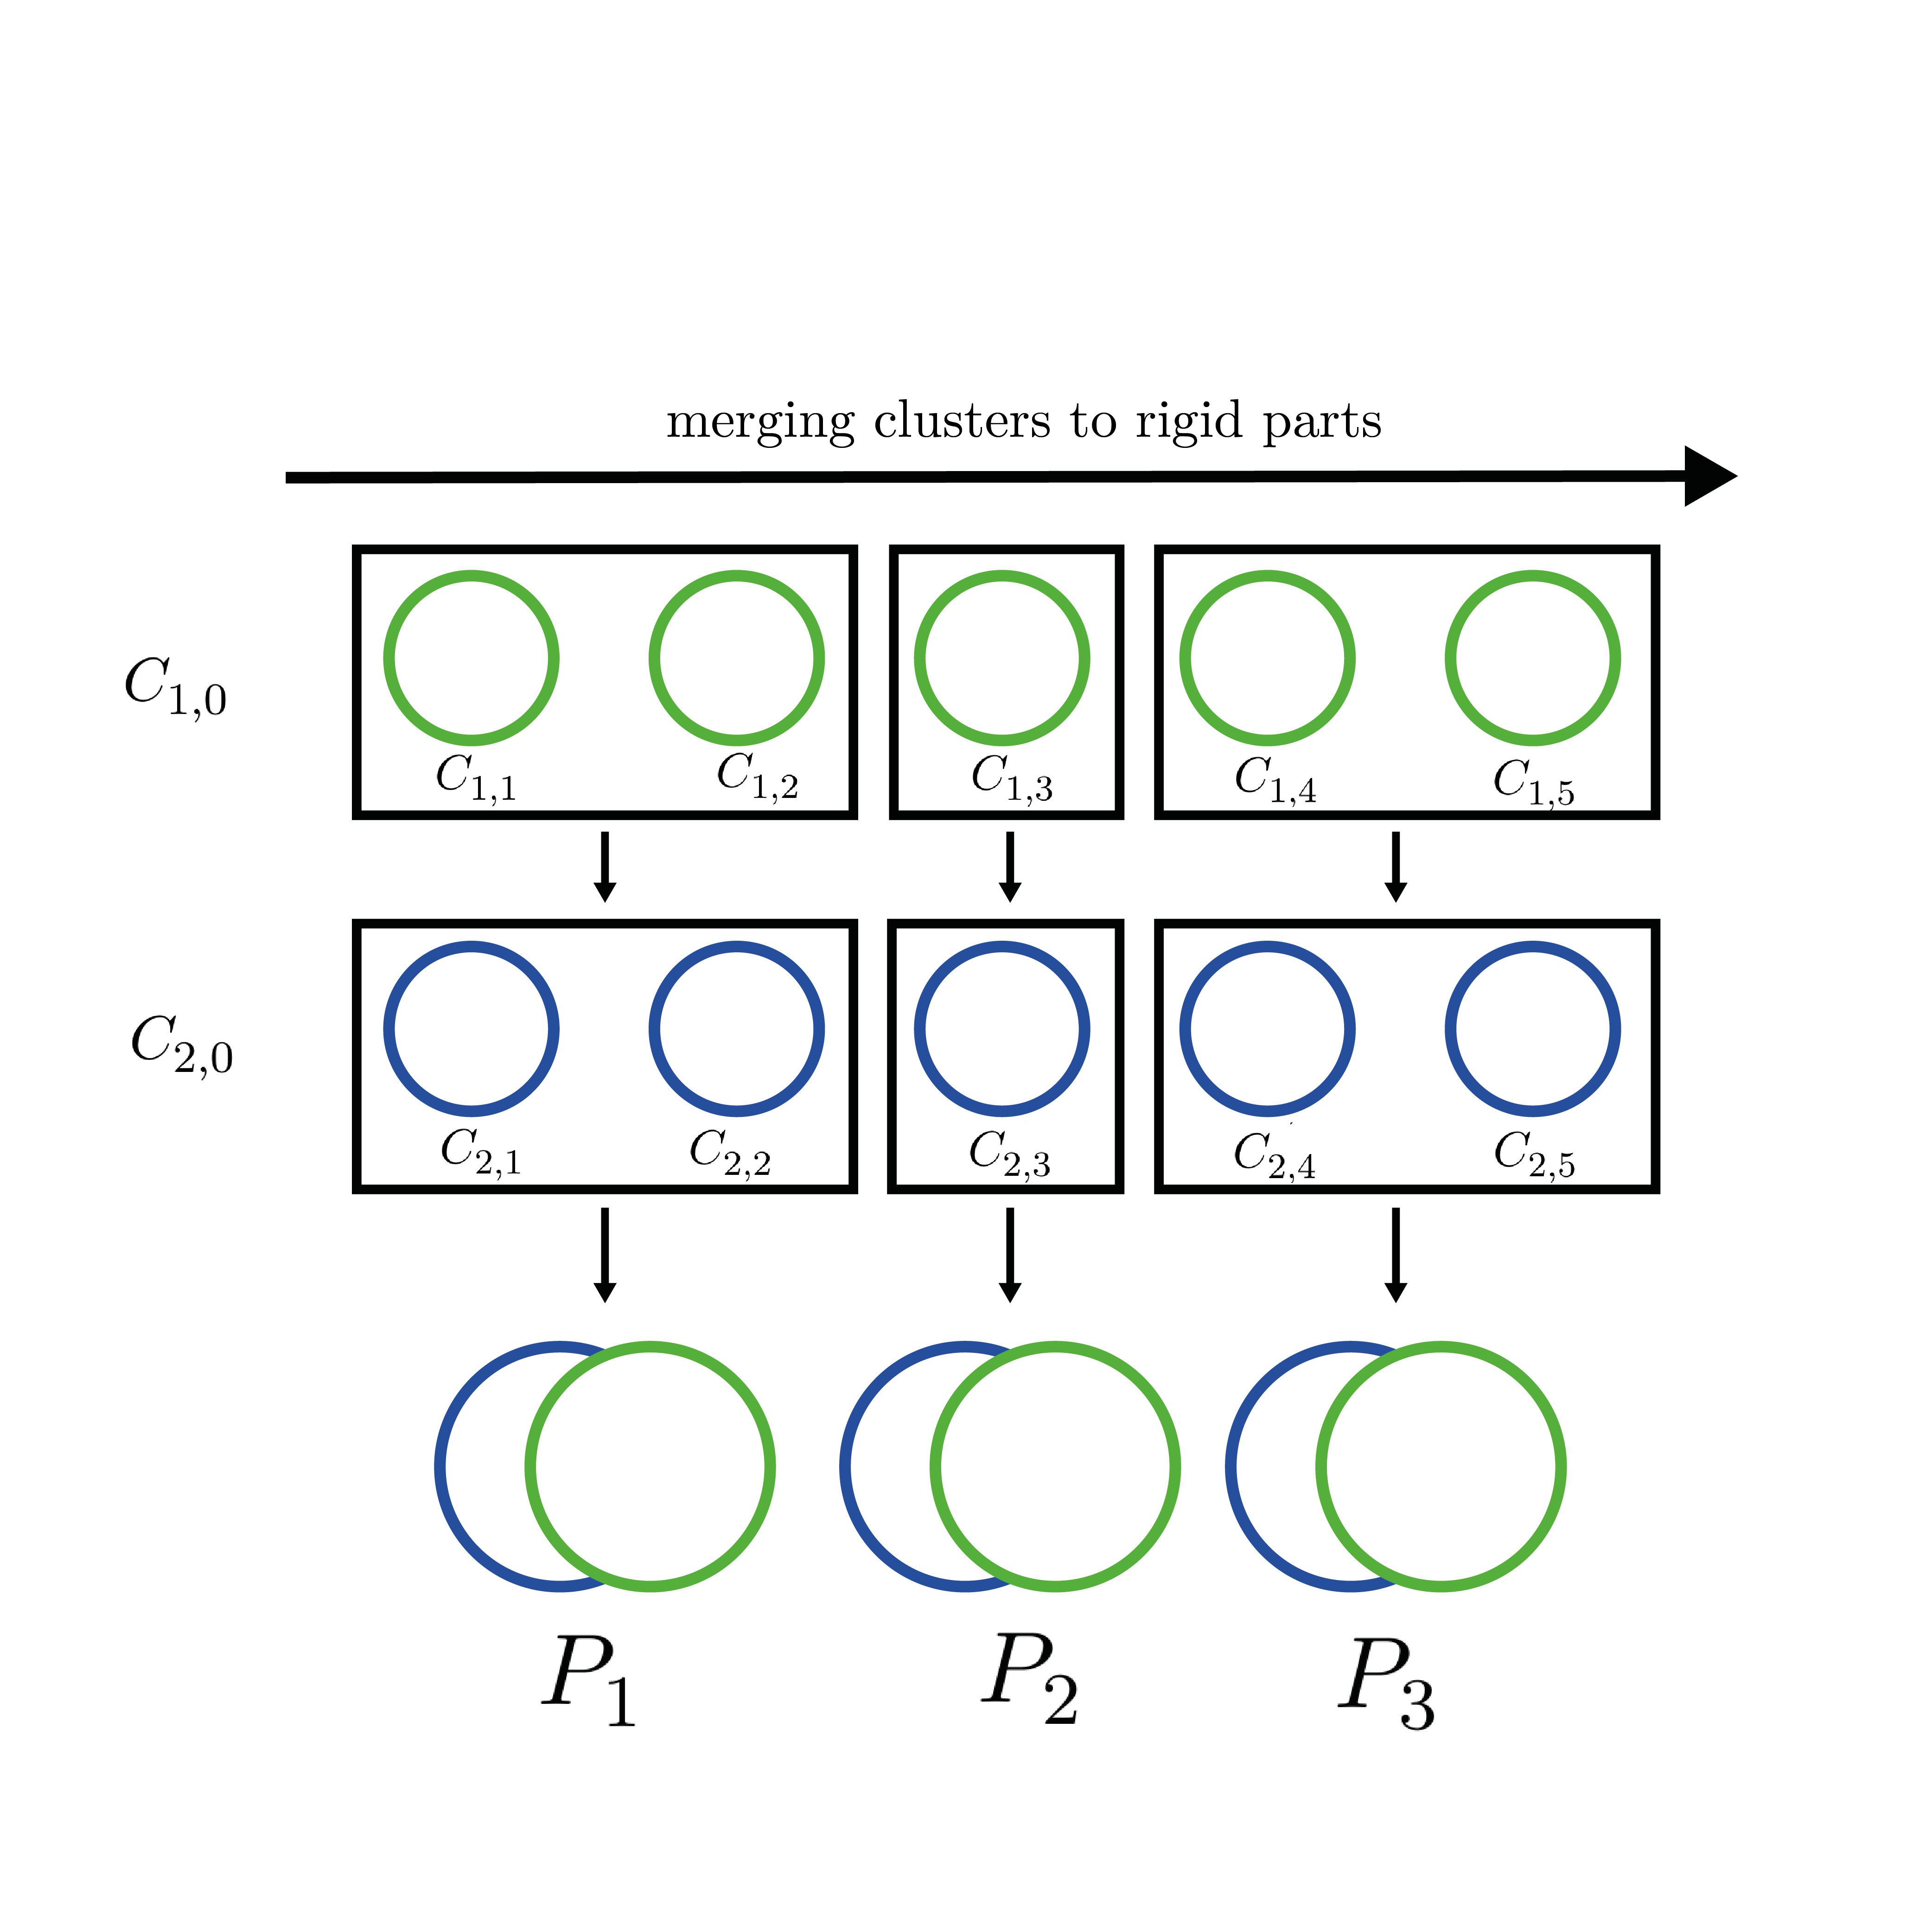
\includegraphics[width=0.8\linewidth]{ClusterChain}
	\caption{Detecting rigid parts of $C_1$ and $C_2$ by iteratively merging neighboring clusters of $C_l$ that merged clusters still match.}
	\label{fig:clusterChain}
\end{figure}

\subsection{Joint/skeleton estimation}

After detecting the rigid parts $\mathcal{P} =  \{ {P_1,....P_m}\}$, they are linked with joints. Their locations are thereby calculated by computing the points of intersection of all principal axis of $\mathcal{P} =  \{ {P_1,....P_m}\}$. However, this calculation assumes that the rigid parts are symmetric, as in the other case the principal axis might not represent the skeleton of an object. For this reason another approach has to be taken into account. Anguelov \cite{Anguelov04} declares joints as two points of two neighboring rigid parts that undergo the same transformation $T$. In the current implementation an object point is only allocated to one rigid part $P$. An improvement of the current situation is therefore to select points that are located near a joint allocated to more neighboring rigid parts and from those selected points the location of a joint is computed. 

\begin{figure}[H]
	\centering\small
	\begin{tabular}{cc}
		\fbox{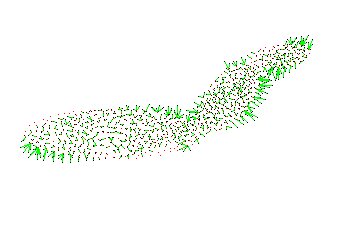
\includegraphics[width=0.45\textwidth]{results/non-rigid_3parts_associations}} &		% JPEG file
		\fbox{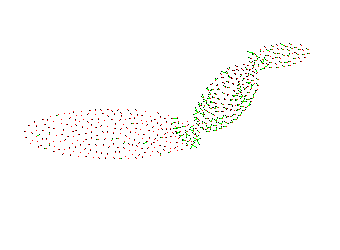
\includegraphics[width=0.45\textwidth]{results/rigid_3parts_associations}} 
		\\	% PNG file
		(a) & (b) 
	\end{tabular}
	\caption{Registration of $C_1$ and $C_2$ before the segmentation into rigid parts (a) and after the segmentation.} 
	\label{fig:ICPResults}
\end{figure}

\chapter{Implementation and Results}

My approach was implemented in Java, using ImageJ as processing library, to focus on implementing and testing the algorithm in 2D. Another implementation is planned in 3D with the PCL to bring the attention to segmentation and visualization in 3D. A class \texttt{Cluster} was implemented to store the cluster's points, its centroid, the orientation $\theta$ as well as the principal and secondary axes. For the subdividing, a \texttt{ClusterTree} was implemented to simultaneously divide the main clusters $C_1$ and $C_2$ into sub clusters (see algorithm \ref{alg:subdivide}). Each node $N$ contains thereby two associated clusters $C_{1,i}$ and $C_{2,i}$. For the clustering and merging of clusters a \texttt{List<Clusters>} was used to dynamically add and remove Clusters. Furthermore, a class \texttt{ICP} was created, which takes two clusters to be matched as input.

\section{Architecture}

The initial algorithm was realized with four classes to divide the own ``divide and conquer'' algorithm from the Cluster object as well as the Visualization and the registration process of sub clusters.
The main class is called ``Segmentation'' which solely requires a stack of two point clouds. First, the noise removal and cluster detection is done in the Cluster class. As a next step, the detected main clusters $m$ $C_1$ $\cdots$ $C_{m}$ are taken as input with an empty list to get the matching sub clusters of all input clusters (see algorithm\ref{alg:inputClusters}). Following, the divide and conquer algorithm (see algorithm \ref{alg:clustering}) takes advantage of the ICP class to iteratively register two sub clusters of two main clusters $C_{i}$ $\cdots$ $C_{j}$. As the segmentation is done depth first the verified sub clusters are stored in the list from left to right. The returned segmented list is taken as input to iteratively merge the sub clusters to detected rigid parts (see algorithm \ref{alg:merging}). As a return we get a list with sub clusters representing the rigid parts of the input clusters. Subsequently, the Visualization class is used, to color the cluster points differently and draw PCA related components, like the axis and interference points of different rigid parts.

\begin{figure}
	\centering
	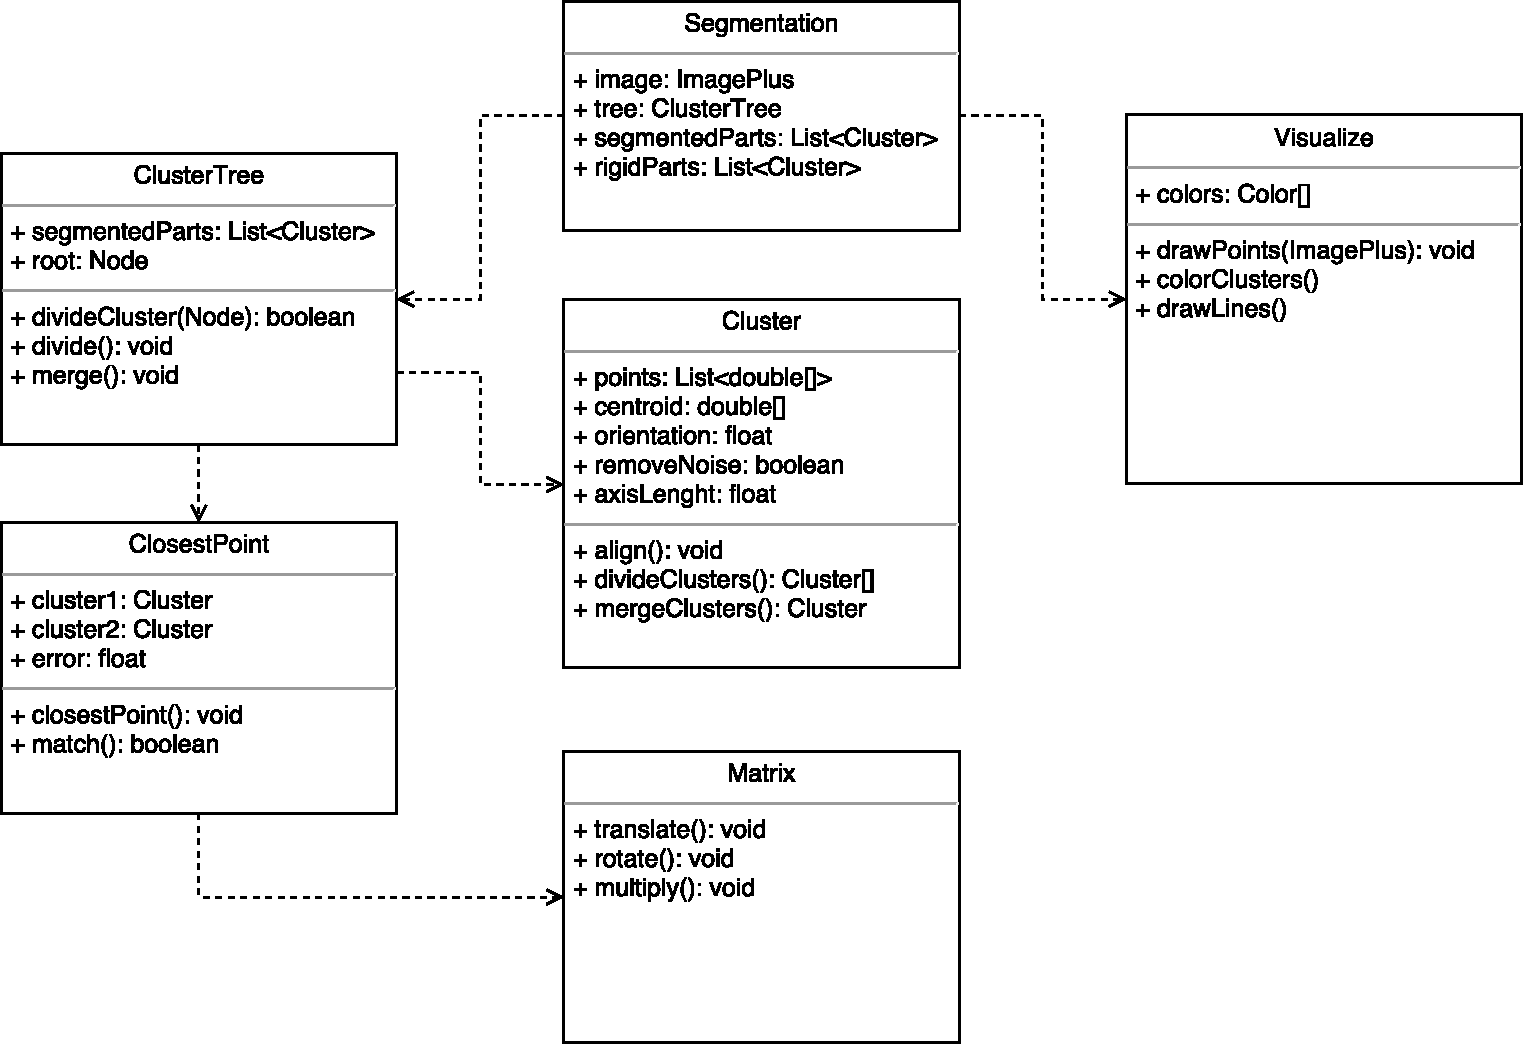
\includegraphics[width=0.9\linewidth]{SegmentationUML}
	\caption{UML diagram of the classes related to the implementation of the algorithm.}
	\label{fig:UML}
\end{figure}

\begin{algorithm}[tbp]
	\caption{Recursive subdividing of two clusters $C_1$ and $C_2$, in the form of a Node $\mathit{N}$ in a Tree, into matching sub clusters. The ICP is applied on two corresponding clusters in $\mathit{N}$ to verify them to match, in which case they are stored in a list. Otherwise, if the two clusters do not match, they are further subdivided. The list with all matching subclusters is returned once the subdivide algorithm terminates.}
	\label{alg:subdivide}
	
		\begin{algorithmic}[1]     % [1] = all lines are numbered
			\label{clusterTree}
			\Procedure{ClusterTree}{$\mathit{C1}, \mathit{C2}$}
			
			\State $\mathit{subclusters} \gets ()$
			\State $\mathit{left} \gets \mathit{nil}$
			\State $\mathit{right} \gets \mathit{nil}$
			\State $\mathit{node:=<C1, C2, left, right>}$
			\State $\mathit{subclusters}$ = \Call{Subdivide}{$\mathit{node}$}
			\State $\mathit{mergedParts}$ =\Call{MergeClusters}{$\mathit{subclusters}$}
			
			\EndProcedure
		\end{algorithmic}
	
	\begin{algorithmic}[1]     % [1] = all lines are numbered
		\label{subdivide}
		\Procedure{Subdivide}{$\mathit{node}$}
		
		\If {\Call{match}{$\mathit{C1(node)}$, $\mathit{C2(node)}$}}
		\Comment{Apply ICP on two clusters}
		\State $\mathit{subclusters = subclusters + (node)}$
		
		\Else
		\State $\mathit{left(node) \gets \Call{Split}{node}}$
		\State $\mathit{right(node) \gets \Call{Split}{node}}$
		\Comment{Split the cluster into a left and right side}
		\State \Call{Subdivide}{$\mathit{left(node)}$}
		\State \Call{Subdivide}{$\mathit{right(node)}$}
		\Comment{Recall the algorithm with sub clusters}
		\EndIf
		
		\State\Return $\mathit{subclusters}$
		\Comment{Return all subclusters after termination.}
		\EndProcedure
			
	\end{algorithmic}
\end{algorithm}

\begin{algorithm}[tbp]
	\caption{Merging of the subclusters of $C_1$ and $C_2$ resulting from algorithm \ref{alg:subdivide} in the order of being stored. Verify the matching of adjacent clusters of $C_1$ and $C_2$ after merging them to one cluster. The merging is continued until no match can be done. In this case the last merging step is reverted and the relevant clusters are stored. The algorithm continues with the next clusters in the list and terminates if all subclusters have been traversed.}
	\label{alg:merging}
	
	\begin{algorithmic}[1]     % [1] = all lines are numbered
		\label{merging}

		\Procedure{MergeClusters}{$\mathit{subclusters}$} 
		\State $\mathit{mergedClusters} \gets ()$
		\State $toBeMergedC1 \gets C1(subclusters[0]$)
		\State $toBeMergedC2 \gets C2(subclusters[0]$)
		
		\For{$i = 1$ to $\mathit{sizeOf(subclusters)}$}
		\State $currentC1 \gets C1(subclusters[i]$)
		\State $currentC2 \gets C2(subclusters[i]$)
		\State $mergedC1 \gets \Call{Merge}{toBeMergedC1, currentC1}$
		\State $mergedC2 \gets \Call{Merge}{toBeMergedC2, currentC2}$
		
		\If {\Call{match}{$\mathit{mergedC1}$, $\mathit{mergedC2}$}}
		\Comment{Apply ICP on two merged clusters}
		\State $\mathit{toBeMergedC1 \gets mergedC1}$
		\State $\mathit{toBeMergedC2 \gets mergedC2}$
		\Comment{Continue merging with merged clusters}
		\Else
		\State $\mathit{mergedClusters = mergedClusters + (toBeMergedC1, toBeMergedC2)}$
		\State $toBeMergedC1 \gets currentC1$
		\State $toBeMergedC2 \gets currentC2$
		\Comment{Initiate merging with current clusters}
		\EndIf
		\EndFor
		\State $\mathit{mergedClusters = mergedClusters + (toBeMergedC1, toBeMergedC2)}$
		\State\Return $\mathit{mergedClusters}$
		\EndProcedure	
	\end{algorithmic}
\end{algorithm}

\section{Intermediate results}

At first, the implementation was tested on two point clouds of an articulated object with only two rigid parts. The segmentation results are directly dependent on the matching error threshold $\tau$ which can bee seen on table \ref{table:segmentation_results}. The higher the threshold $\tau$, the less clusters and subsequently rigid parts can be detected, as two clusters are more likely to match and are not further subdivided. The lower $\tau$, the more clusters and rigid parts will be detected, as clusters require further subdividing in order to match. Figure \ref{fig:2rigidParts} and figure \ref{fig:3rigidParts} show the clustering and rigid part detection of two simple objects, in regard to their rigid parts linked like a chain. For those objects, with a threshold $\tau = 5$ the right number of rigid parts is detected. However, the segmentation position does not correspond to the actual joint of $C_1$ and $C_2$. The reason is, that the average error $e_{avg}$ is computed without any weighting of points. Especially points located near a joint need to be treated cautiously. Figure \ref{fig:4rigidParts} shows a more complex object.
%%
\begin{table}
	\centering\small
	\begin{tabular}{ |c|c|c|c| } 
		\hline
		Rigid parts & $\tau$ & detected clusters & detected rigid parts \\
		\hline
		& 3 & 21 & 14 \\ 
		2& 5 & 3 & 2 \\
		& 7 & 2 & 2 \\
		\hline
		& 4 & 38 & 31 \\ 
		3 & 6 & 4 & 3 \\
		& 8 & 3 & 3 \\
		\hline
		& 6 & 35 & 26 \\ 
		4 & 7 & 3 & 3 \\
		& 8 & 3 & 3 \\
		\hline
	\end{tabular}
	\caption{Segmentation results}
	\label{table:segmentation_results}
\end{table}
%%
\begin{figure}
	\centering\small
	\begin{tabular}{@{}c@{\hspace{2mm}}c@{}} % mittlerer Abstand = 12mm
		\fbox{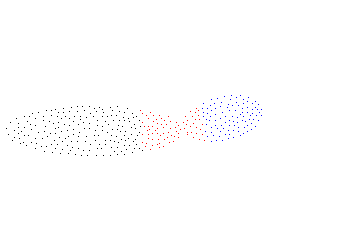
\includegraphics[width=.40\textwidth]{results/2_1parts_clusters_2th}} &
		\fbox{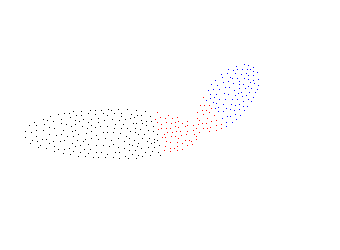
\includegraphics[width=.40\textwidth]{results/2_2parts_clusters_2th}} 
		\\
		(a) & (b)
		\\[4pt]	%vertical extra spacing (4 points)
		\fbox{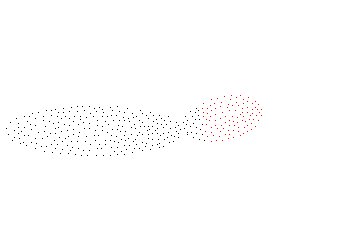
\includegraphics[width=.40\textwidth]{results/2_1parts_rigidParts_2th}} &
		\fbox{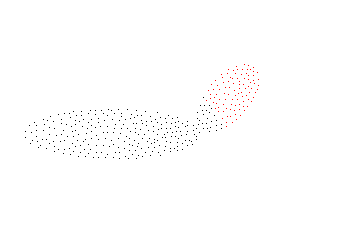
\includegraphics[width=.40\textwidth]{results/2_2parts_rigidParts_2th}} 
		\\
		(c) & (d)
	\end{tabular}
	\caption{Taking a Mesh $M$ in two poses with only two rigid parts as input, with a threshold $\tau = 5$, 3 clusters are detected in $C_1$~(a) and $C_2$~(b),
		which results in 2 rigid parts in $C_1$~(c) and $C_2$~(d).}
	\label{fig:2rigidParts}
\end{figure}
%%
\begin{figure}
	\centering\small
	\begin{tabular}{@{}c@{\hspace{2mm}}c@{}} % mittlerer Abstand = 12mm
		\fbox{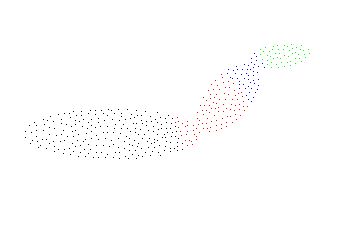
\includegraphics[width=.40\textwidth]{results/3_1parts_clusters_2th}} &
		\fbox{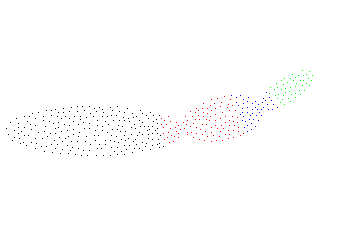
\includegraphics[width=.40\textwidth]{results/3_2parts_clusters_2th}} 
		\\
		(a) & (b)
		\\[4pt]	%vertical extra spacing (4 points)
		\fbox{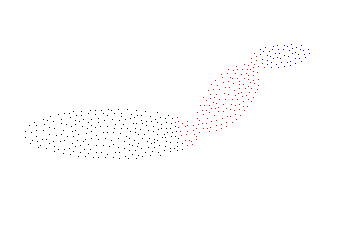
\includegraphics[width=.40\textwidth]{results/3_1parts_rigidParts_2th}} &
		\fbox{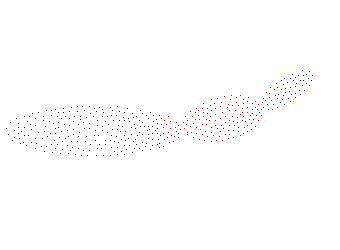
\includegraphics[width=.40\textwidth]{results/3_2parts_rigidParts_2th}} 
		\\
		(c) & (d)
	\end{tabular}
	\caption{Taking a Mesh $M$ in two poses with three rigid parts as an input, with a threshold $\tau = 6$, 4 clusters are detected in $C_1$~(a) and $C_2$~(b),
		which results in 3 rigid parts in $C_1$~(c) and $C_2$~(d).}
	\label{fig:3rigidParts}
\end{figure}
The segmentation into rigid parts is also apparent, when visualizing the point registration between $C_1$ and $C_2$ (see figure \ref{fig:ICPResults}). Two associated points from $C_1$ and $C_2$ are thereby linked with green lines. Comparing the registration results before and after a segmentation into rigid parts clearly shows, that the registration of rigid parts with the ICP results in a lower matching error $e$.
%%	
\begin{figure}[H]
	\centering\small
	\begin{tabular}{cc}
		\fbox{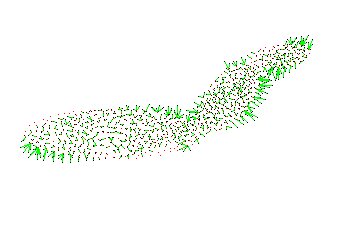
\includegraphics[width=0.45\textwidth]{results/non-rigid_3parts_associations}} &		% JPEG file
		\fbox{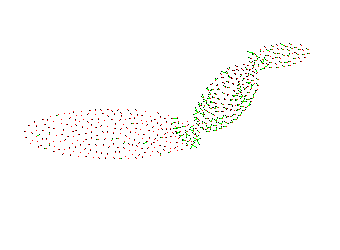
\includegraphics[width=0.45\textwidth]{results/rigid_3parts_associations}} 
		\\	% PNG file
		(a) & (b) 
	\end{tabular}
	\caption{Registration of $C_1$ and $C_2$ before the segmentation into rigid parts (a) and after the segmentation (b).} 
	\label{fig:ICPResults}
\end{figure}
%%		
In case of a more complex object, the simple segmentation algorithm fails. Although varying threshold $\tau$ for the matching, there are either too many or few rigid parts detected. When using $\tau = 7$ (see figure \ref{fig:4rigidPartsHighTH}) only 3 clusters and rigid parts can be detected. By decreasing $\tau$ to 6 (see Figure \ref{fig:4rigidParts}), further subdividing is done, which leads to a too high number of rigid parts and clusters.
%%
\begin{figure}[H]
	\centering\small
	\begin{tabular}{cc}
		\fbox{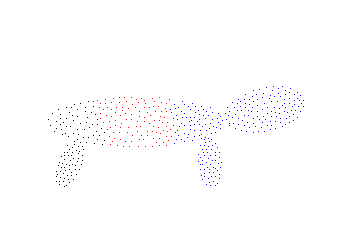
\includegraphics[width=0.45\textwidth]{results/4_1parts_clusters_rigidParts_7th}} &		% JPEG file
		\fbox{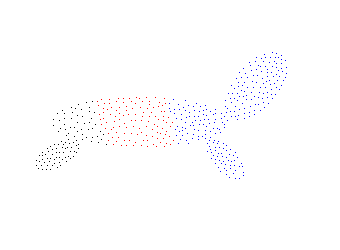
\includegraphics[width=0.45\textwidth]{results/4_2parts_clusters_rigidParts_7th}} 
		\\	% PNG file
		(a) & (b) 
	\end{tabular}
	\caption{Taking a more complex Mesh $M$ in two poses with four rigid parts as an input, with a threshold $\tau = 7$, 3 clusters and rigid parts can be detected in $C_1$~(a) and $C_2$~(b).} 
	\label{fig:4rigidPartsHighTH}
\end{figure}
\begin{figure}[H]
	\centering\small
	\begin{tabular}{@{}c@{\hspace{2mm}}c@{}} % mittlerer Abstand = 12mm
		\fbox{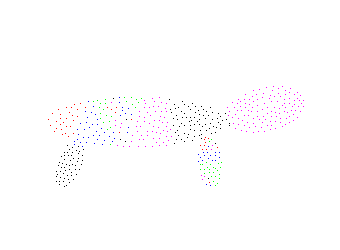
\includegraphics[width=.40\textwidth]{results/4_2parts_clusters_6th}} &
		\fbox{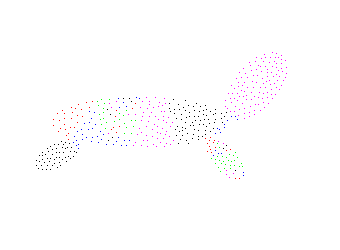
\includegraphics[width=.40\textwidth]{results/4_1parts_clusters_6th}} 
		\\
		(a) & (b)
		\\[4pt]	%vertical extra spacing (4 points)
		\fbox{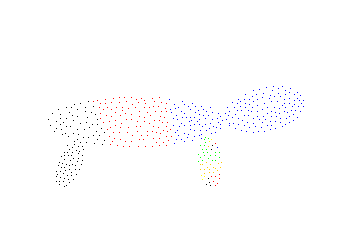
\includegraphics[width=.40\textwidth]{results/4_1parts_rigidParts_6th}} &
		\fbox{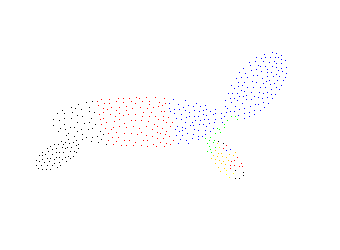
\includegraphics[width=.40\textwidth]{results/4_2parts_rigidParts_6th}} 
		\\
		(c) & (d)
	\end{tabular}
	\caption{Taking a more complex Mesh $M$ in two poses with four rigid parts as an input, with a threshold $\tau = 6$ , 35 clusters are detected in $C_1$~(a) and $C_2$~(b),
		which results in 26 rigid parts in $C_1$~(c) and $C_2$~(d).}
	\label{fig:4rigidParts}
\end{figure}	
The algorithm generally works for simple objects, in which the rigid parts are linked like a chain. Still, the segmentation location is not accurate, which might be disposed by introducing weights to points located near a joint. For more complex object with a skeleton structure, e.g. a human, where one rigid part is linked to more than two rigid parts, this simple implementation fails. In this case, another approach has to be found, as a skeleton structure is more complex to extract than a simple chain structure.

\chapter{Improvements}

In case of objects with a skelton structure, the segmentation algorithm in its simple form fails. As a result, the approach needs to be extended. Additionally, for simple objects the detection of the joints is not exact although the segmentation to the approximate rigid parts works. Also for that improvements have to be done, which for example include the special treatment for points located near to a joint.

\section{Region growing}
During the segmentation of an object in two different poses having the same number of points, there is the general case that the divided parts being compared do not contain the same number of points. As this state might come to undesirable matching errors, parts with the same sizes could be generated by region growing. e.g. by starting with the most outside point of two poses and grow regions with the same size of points which are then compared. The points being grown would then account to the minimum size of two subclusters of $C_1$ and $C_2$. Furthermore, the detection of multiple clusters could be treated, in case of subdividing clusters. A similar approach was taken during the LRP algorithm \cite{guo2016correspondence}. The detected clusters are as a result treated individually.

\section{Matching error}
Another improvement possibility would be to ensure that during the ICP procedure each point only has one nearest neighbor and also considering the case, that there are not always the same amount of points in two clusters. By doing so, not all points would contribute to the matching error. Furthermore, weights should be added to the points, especially points located near a joint should be treated cautiously. A cluster could be therefore further subdivided, if a minimum number of points is above the error threshold $\tau$ and not the average. 
%%
%TODO: TEST RESULTS!
%%
Implementing those improvements, the algorithm can be considerably improved for simple objects tested before. But still, further considerations have to be done for articulated objects.


\chapter{Implementation in 3D}

After checking the algorithm in 2D, it was implemented in 3D using the PCL. There are already a number of methods available, like registration with the ICP and PCA related components.
\chapter{Improvements}

In case of articulated objects with a skeleton structure, the segmentation algorithm in its simple form fails. The main reasons are the following:
%%
\begin{itemize}
	\item By recursively subdividing $C_1$ and $C_2$ the detected sub clusters might actually count to more than one and being located apart from each other. 
	\item In case of a matching cluster being a part of a rigid part, no further operations are done with the match. The rigid part is anticipated to be generated by merging neighboring sub clusters.
	\item By further sub dividing clusters, the merging becomes more difficult, as the clusters are scattered next to each other.
	\item The detection of joints is not exact although the segmentation in the approximate rigid parts succeeds as sub clusters are good enough to fit, but still there might be better fits with less or more points.
\end{itemize}
%%
Thus, the initial approach needs to be extended, which solved the issues being mentioned.

\section{Region growing}
During the segmentation of an object in two different poses, there is the general case that the divided parts being compared do not contain the same number of points. As this state might come to undesirable matching errors, parts with the same sizes could be generated by region growing. This can be e.g. implemented by starting with the most outside point of two poses and grow regions with the same size of points which are then compared. Furthermore, the detection of multiple clusters can be treated, in case of subdividing clusters. The detected clusters are as a result treated individually.

\section{Matching error}
Another improvement is the assurance that during the ICP procedure each point only has one nearest neighbor and also considering the case, that there are not always the same amount of points in two clusters (uneven number of points). By doing so, not all points would contribute to the matching error. Furthermore, weights should be added to the points, especially points located near a joint should be treated cautiously. A cluster could be therefore further subdivided, if a minimum number of points is above the error threshold $\tau$ and not the average. 

%\section{Initial alignment of clusters}
%The initial ``Divide and Conquer'' approach is used to detect two matching sub clusters of $C_1$ and $C_2$. But unlike previous implementations, the rigid parts are not detected by a following merging step, but by region growing, until the matching error $e$ is above the specified threshold $\tau$.
%If a rigid part is detected, it is stored and the same procedures initiates with the other points of $C_1$ and $C_2$. By doing so, all rigid parts are sequentially detected from one direction to the other.

%\subsection{Error handling}
%The region growing procedure needs to terminate if points of another rigid part are added. Following, a higher matching error $e$ is detected. To guarantee successful rigid part detection this procedure premises that the regions in two comparing sub clusters grow the same way, otherwise the region growing might terminate before detecting the whole rigid part. 

\section{Segmentation of articulated objects}
The most crucial deficit  of the proposed algorithm is that is does not work with articulated objects, whose parts are not simple linked as a chain, but a rigid part can have more than two linking rigid parts. An example would be the skeleton of humans and most animals. As a result, the objects are simply too complex to linearly subdivide them. One improvement proposition is thereby the initial alignment of the object, that the largest rigid part is aligned.  A similar approach was taken during the LRP algorithm \cite{guo2016correspondence}. Then, recursively linked parts of this largest rigid part are detected (see section \ref{LRP}).

\section{Largest rigid part}
\label{LRP}

As opposed to recursively subdividing $C_1$ and $C_2$ into sub clusters, as an initial step the largest rigid part (LRP) is detected. From there, all other linked parts can be detected by region growing and reapplying the algorithm.
The algorithm was applied on 3D point clouds by \ref{LRP}.

\subsection{Basic functionality}
\label{functionalityLRP}
As an initial step, the LRP algorithm  attempts to detect the most reliable correspondences between $C_1$ and $C_2$. For that, local descriptors (FPFH) are computed. The requirement for a sparse correspondence between two cluster points $\boldsymbol{p}_i(x,y)$ and $\boldsymbol{p}_j(x,y)$ is that they are \textit{reciprocal}, which means that two points $\boldsymbol{p}_i(x,y)$ and $\boldsymbol{p}_j(x,y)$ are the most similar from each other. Some of the sparse correspondences are assumed to be wrong. Therefore, by applying RANSAC to the point correspondences, a single rigid transformation is aimed for to detect the so-called ``largest rigid part'' (LRP), which is supported by the largest corresponding point cluster between $C_1$ and $C_2$. In case of a human, this would be the torso. Subsequently, all linked rigid parts to the LRP are detected by recursively applying the algorithm on grown clusters from the current LRP.

\subsection{Implementation steps}

In order to re-implement the algorithm in 2D, modifications had to be accomplished. The most crucial part of the whole algorithm is the initial alignment of $C_1$ and $C_2$ in order to detect the actual largest rigid part of the articulated object. This step is of particular importance, as the subsequent detection of further rigid parts proceeds from there. Therefore, as first step, sparse correspondences between $C_1$ and $C_2$ have to be detected (see subsection \ref{correspondences}). The initial idea was to detect correspondences by applying the ICP only proceeding the iterative transformation calculation with the most reliable correspondences. However, this approach did not manage to detect the desired correspondences of the largest rigid part (see section \ref{ResultsLRP}). Building on the reference paper by Mitra \cite{Mitra07} features for all points of $C_1$ and $C_2$ are computed to use those for point correspondences between two clusters $C_1$ and $C_2$.

\begin{enumerate}
	\item The PCA is employed on the input clusters $C_1$ and $C_2$ to estimate normals of all points.
	\item Point features are computed to detect sparse point correspondences between $C_1$ and $C_2$. A Point correspondence between $C_1$ and $C_2$ needs to be \textit{reciprocal}.
	\item The RANSAC approach is applied on those correspondences to detect a $T_j$ that rejects wrong point correspondences. Clusters are detected from all corresponding points by applying region growing.
	\item The LRP is assigned to the resulting biggest point cluster.
	\item Proceeding with the LRP, unmatched clusters to $C_1$ and $C_2$ are seeked by region growing from the LRP. The algorithm is then reapplied on those clusters until all rigid parts have been discovered.
\end{enumerate}

\subsection{Detection of sparse correspondences}
\label{correspondences}

\subsubsection{ICP}
Sparse correspondences of two input clusters $C_i$ and $C_j$ were initially achieved by applying the Iterative closest point algorithm. Thereby, the two input clusters are aligned by means of the PCA. Following, corresponding points of $C_i$ and $C_j$ are only considered, if they are \textit{reciprocal} (see subsection \ref{functionalityLRP}). Furthermore, the euclidean distance between two cluster points $d(\boldsymbol{p}_i,\boldsymbol{p}_j)$ must be below a predefined threshold $\tau$. As a consequence, points being located far away from each other do not contribute to the alignment of $C_i$ and $C_j$ and are not stored as correspondence. Those are assumed to be small rigid parts with different transformations.

\subsubsection{Point features}
As the intermediate results of the detection of the largest rigid part when applying only the ICP were insufficient for further computations (see section \ref{ResultsLRP}) another approach had to be applied. As proposed in \cite{Mitra07} a fast point feature histogram \cite{FPFH} was implemented in 2D. It is an improved approach of the `'Persistent Point Feature Histogram for 3D Point Clouds'' \cite{PPFH}. The choice of those features are the following: 
%%
\begin{itemize}
	\item rotation-invariant features
	\item easy comparison of features
	\item low complex implementation
\end{itemize}
%%
By using a histogram the neighborhoods' geometrical properties can be provided in form of the mean surface curvature at a point $\boldsymbol{p}$. As a first step, the normals of all points from the input clusters $C_1$ and $C_2$ need to be estimated. Those is achieved by taking all points within a radius $r$ from a point $\boldsymbol{p}$. The normals need to be re-oriented and are calculated by using the approach from \cite{normals}. The simplified point feature histogram (SPFH) for a point $\boldsymbol{p}$ is then computed by using three geometric features. Between $\boldsymbol{p}$ and each of its $n$ neighbors $\boldsymbol{p_n}$ given a threshold $\tau$, those features are computed -- $\boldsymbol{p_i}$ is thereby the point having the smaller angle between its normal and the line connecting the point set, $\boldsymbol{p_j}$ the remaining point. Using their normals $n_i$ and $n_j$ a Darboux $uvn$ frame $(u = n_i, v = (p_j - p_i) \times u, w = u \times v)$ is computed. The following angles
%%
\begin{equation}
\begin{split}
\alpha = v \cdot n_j
\\
\phi = (u \cdot (p_j - p_i))/\|p_j - p_j\|
\\
\theta = arctan(w \cdot n_j, u \cdot n_j)
\end{split}
\label{eq:AngularVariations}
\end{equation}
%%
are computed. In a second step for each point $\boldsymbol{p_i}$ again all $n$ neighbor points given a threshold $tau$ are computed. The final histogram of $p$ is then weighted to the final histogram (FPFH)
%%
\begin{equation}
FPFH(\boldsymbol{p}) = SPF(\boldsymbol{p}) + \frac{1}{n} \cdot \displaystyle\sum_{i=1}^{n}\frac{1}{w_i} \cdot SPF(p_i)
\end{equation}
%%
where the weight $w_i$ represents the distance $d(\boldsymbol{p},\boldsymbol{p}_i)$. The influence region diagram for a Fast Point feature histogram for a query point $\boldsymbol{p_q}$ can be seen on Figure \ref{fig:FPFHregion}. 
%%
\begin{figure}[H]
	\centering
	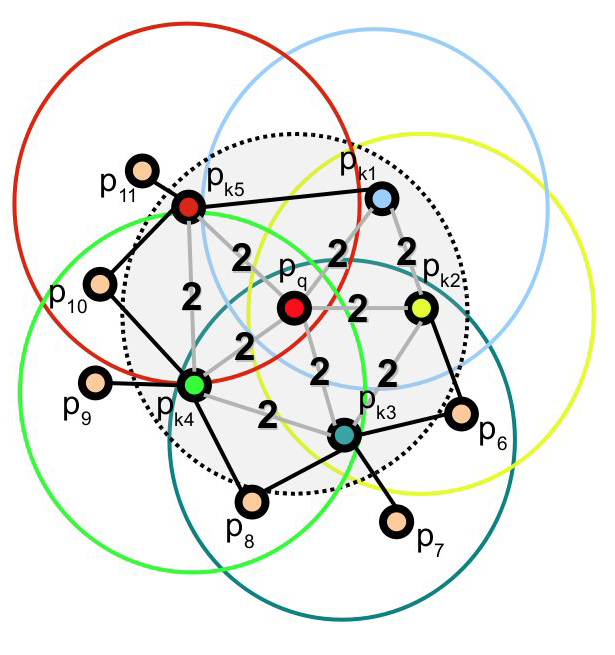
\includegraphics[width=0.4\linewidth]{FPFH_region}
	\caption{The point region for the calculation of the feature histogram for a query point $\boldsymbol{p}_q$. The histogram of $\boldsymbol{p}_q$ and its neighbors (inside the grey circle) is weighted with the further linked neighbors (colored circles).}
	\label{fig:FPFHregion}
\end{figure}
%%
The resulting features are added into histograms with 125 bins. As soon as the feature histograms of all points from $C_1$ and $C_2$ are computed, they can be compared and the most similar histograms are selected as correspondence if they are \textit{reciprocal}. Before, a persistence analysis is computed, which only takes salient histograms for comparison. 

\subsection{Detection of the largest rigid part}
\label{detectionLRP}
The dense point correspondences from the previous computation step (see subsection \ref{correspondences}) may contain several errors. Therefore, RANSAC is applied as a next step to detect a single rigid transformation $T$ that leads to the biggest overlapping point cluster of $C_i$ and $C_j$. Thereby, in each iteration, 3 random correspondences are selected and used for the calculation of $T$ which is applied on $C_i$ to be translated on $C_j$. Subsequently, clusters are grown from all corresponding points with an euclidean distance $d(\boldsymbol{p}_i,\boldsymbol{p}_j)$ again below a predefined threshold $\tau$. The procedure is applied both on $C_i$ and $C_j$ which results in two rigid parts as output. In case of symmetric poses, the RANSAC would not be required, as the largest rigid part (the torso) would be almost perfectly aligned and taken as input for the region growing. But still, to cover as many cases as possible, this computation step is necessary. 

\subsection{Cluster detection by region growing}
\label{cluster}
After successfully detecting a ``largest rigid part'' $P_i$ and $P_j$ for each input clusters $C_i$ and $C_j$ they are added to a list of rigid parts $\mathcal{P}$. Potential linked rigid parts are detected from region growing of all unclustered points $\mathcal{U} =  \{\boldsymbol{u}_1,\ldots,\boldsymbol{u}_n\}$. Those comprise all cluster points of $C_1$ and $C_2$ excluding already detected largest rigid parts $\mathcal{P}$. The region growing initiates with the first point $\boldsymbol{u}_1$ of the unclustered points $\mathcal{U}$ to form a cluster $C_i$. Another point of the unclustered points $\boldsymbol{u}_j$ is added to $C_i$, if the euclidean distance $d(\boldsymbol{p}_i,\boldsymbol{u}_j)$ to any point in $C_i$ is below the threshold $\tau$. If no further unclustered points can be added, the region growing initiates again with the first unclustered point $\boldsymbol{u}_1$ that has not been added by region growing until all points traversed the procedure. The result is a set of clusters $\mathcal{C}$ for each $C_i$ and $C_j$. Subsequently, a preliminary joint $\boldsymbol{j}_i$ for each output clusters is stored, by detecting the two nearest points of $C_i$ and $P_i$. The joints are required for following cluster correspondence and joint weights for the ICP (see subsection \ref{CorrespondingClusters} and \ref{JointWeights}).

\subsection{Establishment of corresponding clusters}
\label{CorrespondingClusters}
In case of detecting more than one cluster for each $C_i$ and $C_j$, which might be for example the case for the extremities linked to the torso, it must be verified which clusters correspond to each other. This step is essential, as the algorithm is called recursively (starting from \ref{correspondences}) with two new input clusters. Thereby, the provisional joints $\boldsymbol{j}_i$ are used to associate two clusters of $C_i$ and $C_j$ by detecting the closest joint with the euclidean distance $d(\boldsymbol{j}_i,\boldsymbol{j}_j)$.

\subsection{Joint weights}
\label{JointWeights}
In order to iteratively detect largest rigid parts that are actually linked to another detected ``largest rigid part'', the preliminary joints resulting from \ref{cluster} are used as weights. Thereby, points being located far away from joints, do not contribute as much to the matching error as point located near a joint. By doing so, joint consistency across two poses is enforced. As an alternative to the ICP clusters with calculated joints only need to be rotated around them. As a result, a matching error $e$ 
%
\begin{equation}
	e = \displaystyle\sum_{i=1}^{m}\| \boldsymbol{p}_i - \boldsymbol{q}_i\|^2 \cdot \| \boldsymbol{p}_i - \boldsymbol{j}_i\|
\end{equation}
%
is achieved which combines the distance to the closest point and to the cluster's joint. Thereby, not only successful correspondences are taken as input but all points, that the error is expressive. The final correspondence equals to the rotation around the joint $\boldsymbol{j}_i$ with the smallest error $e$. 

\section{Implementation}
\label{ImplementationLRP}
The individual steps of the largest rigid part algorithm have also been split in the implementation for better overview. 
%
%TODO: Add code snippets to implementation LRP
%
\subsection{ICP}
One main part of the algorithm is the modified implementation of the ICP using Procrustes fitting to compute a transformation that detects sparse point correspondences. Thereby, only reciprocal correspondences within a specific distance $\tau$ contribute to the calculation. The final point correspondences of $C_i$ and $C_j$ are stored in a \texttt{Map<Integer, Integer>} containing the indices of the corresponding points. This is because the storage of points in the form $\boldsymbol{p}_i(x,y)$ would underly a specific transformation, which is applied during the ICP and initial alignment. For further computations using the RANSAC, no transformations are desired. As the main difficulty is the right initial alignment of the actual largest rigid part (torso) the value of the distance threshold $\tau$ is chosen generously. As a result, a higher number of false point correspondences is detected which has to be compensated by RANSAC (see subsection \ref{RANSAC}).

\begin{lstlisting}
...
for (Map.Entry<Integer, Integer> entry : reference.entrySet()) {
Integer referenceIndex = entry.getKey();
Integer targetIndex = entry.getValue();

	if (target.containsKey(targetIndex) && target.get(targetIndex) == referenceIndex) {
		referencePoints.add(originalReference.get(referenceIndex));
		targetPoints.add(originalTarget.get(targetIndex));
		finalAssociations.put(referenceIndex, targetIndex);
	}
}
...
\end{lstlisting}

\subsection{Image Features}
%
%TODO: implementation of features (incl normals)
%
\subsection{RANSAC}
\label{RANSAC}
The RANSAC algorithm takes the computed dense correspondences between $C_i$ and $C_j$ in form of a \texttt{Map<Integer, Integer>} as input. As a first step, three random correspondences are selected from the map to calculate an affine transformation between the three resulting points from each $C_i$ and $C_j$. The initial orientation and alignment is thereby irrelevant as the transformation $T$ is completely recalculated.

\begin{lstlisting}
public LargestRigidPart(Cluster c_i, Cluster c_j, Map<Integer, Integer> correspondences)
...
points1 = c_i.getPoints();
points2 = c_j.getPoints();
...
private void getRandomPoints(int num) {
	Integer[] keys = correspondances.keySet().toArray(new Integer[0]);
	Integer[] values = correspondances.values().toArray(new Integer[0]);

	for (int i = 0; i < num; i++) {
		index = (int) (Math.random() * correspondances.size());
		randomPoints1.add(points1.get(keys[index]));
		randomPoints2.add(points2.get(values[index]));
	}
}
...
\end{lstlisting}

Similar to the ICP, a closest point procedure with a threshold $\tau$ is conducted. The value is thereby considerably smaller than in the ICP as a right alignment during any iteration is assumed. Unlikely the ICP, no error during the Procrustes fit is accumulated, instead the detected point correspondences are taken as input in the region growing \ref{RegionGrowing} procedure. The biggest cluster is stored and after all iterations returned as largest rigid part.

\subsection{Region growing}
\label{RegionGrowing}
The region growing algorithm is quite similar to the earlier described algorithm (see algorithm \ref{noiseRemoval}). There is also an adaptation, which does not only return the largest cluster, but all clusters above a certain size. The detected clusters are handled in a \texttt{Stack<Cluster>} in case of more than one detected clusters. Thereby, all clusters are pushed on the stack. With each recursion two corresponding cluster $C_i$ and $C_j$ are popped from the stack and taken as input for the whole algorithm. If again more clusters are detected they are pushed on the stack and treated before recently added clusters.

\section{Results}
\label{ResultsLRP}

As the input point cloud of an articulated object is in 2D, the imitation of the object's hull is required. As a consequence, the region growing is much more error-prone, as unlikely in 3D, the points of a rigid part have a considerable lower number of neighbors. In case of a few missing cluster points from a rigid part, it will not be fully detected during the region growing due to the gaps. To counteract this behavior, joints are added to each rigid part, that more links for region growing are available. 

%TODO: add pictures of LRP results

The first main difficulty is the first alignment of the two input clusters $C_1$ and $C_2$. As the execution of the algorithm is only dependent on a succesful alignment, for test cases the assumption was made, that the orientation of the two poses are initially right. The main drawback of the ICP was that the starting position of the two main clusters $C_1$ and $C_2$ had to be ideal that the largest rigid part could be detected. However, this could not be guaranteed as asymmetrical body poses would influence the orientation (see Figure XXX) of the whole cluster $C_1$. As a result, reciprocal point correspondences could not be detected that would lead to the largest rigid part.

\subsection{Main drawbacks}
The main drawback of the algorithm represents the first initial alignment of the two poses of the articulated object. Thereby, it is directly dependent on the symmetry of the pose. The less symmetry the higher the changes that the initial alignment on the largest rigid part might fail. The reason is that the ICP expects a good starting alignment. As it is assumed that the major largest rigid part contributes most to the principal axis and the initial alignment, it would work. But in case of an unbalance of the linked parts, the alignment of the LRP might shift in a certain direction and it might not be detected during the ICP. As a result the whole algorithm fails. Furthermore, touching of rigid parts (e.g. the hand touches the leg) constitute difficulties as the region growing would not detect those as potential linked clusters. 

\subsection{Possible solutions}

A possible solution to the main drawbacks is the usage of point features for the initial alignment. Those are more reliable across two poses than the anticipated symmetry of the points on linked parts. A similar implementation was done in 3D by Mitra \cite{Mitra07} (see section \ref{functionalityLRP}). 

%TODO: Write what fails/main problems/solutions








\chapter{Implementation in 3D}

After checking the algorithm in 2D, it was implemented in 3D using the PCL. There are already a number of methods available, like registration with the ICP and PCA related components.
\chapter{Conclusion}
\label{cha:Closing}

In the first project phase, intense research has been conducted in order to detect one main issue to focus on in the master project. For that, it was quite essential to form an overall perspective of the state-of-the-art regarding motion and pose estimation. During this process, the field of unsupervised pose estimation frequently arose. By following this direction, the non-rigid registration became a major indicator for possible optimizations. Taking existing methods as reference (see Chapter \ref{cha:RelatedWork}), an own approach for 2D point clouds was developed, which should reduce the computation steps of detecting the rigid parts of an articulated non-rigid object. Basically, a divide-and-conquer approach was developed, which recursively divides two point-clouds of the same object in different poses into matching clusters. The subdividing was realized with a tree and depth-first traversal to segment the point clouds from the left to the right. As a next step, all neighboring clusters were verified to be merged, in case of having subdivided a rigid part. After the merging the rigid parts of the objects are detected. 

%TODO: what has been achieved? --> Results 



%TODO: major difficulties, problems




%TODO: what can be further done
	
\section{Future work}

Machine learning of feature histograms \cite{surfletPairRelation}.

%TODO: 3D implementation?


%%%----------------------------------------------------------
\appendix                                         % appendix 
%%%----------------------------------------------------------

%\chapter{Technical Details}
\label{app:TechnicalDetails}



	% technical supplements
%\chapter{CD-ROM/DVD Contents}
\label{app:cdrom}


	% contents of the CD-ROM/DVD
%\chapter{Change History}
\label{app:ChangeHistory}





	% chronological list of changes
%\chapter{\latex Source Code}
\label{app:SourceCode}

	% source text of this document

%%%----------------------------------------------------------
\MakeBibliography                        				% references
%%%----------------------------------------------------------

%%% special page for checking print size --------------------
%\chapter*{Check Final Print Size}

\begin{center}
{\Large --- Check final print size! ---}

\bigskip

\calibrationbox{100}{50} % width/height of box in mm

\bigskip

{\Large --- Remove this page after printing! ---}

\end{center}



%%%----------------------------------------------------------
\end{document}
%%%----------------------------------------------------------